%%%  کلاس AUTthesis، نسخه آبان 1397
%%%   دانشگاه صنعتی امیرکبیر                 http://www.aut.ac.ir
%%%  تالار گفتگوی پارسی‌لاتک،       http://forum.parsilatex.com
%%%   آپدیت شده در آبان 95
%%%   پشتیبانی و راهنمایی          badali_farhad@yahoo.com
%%%
%%%   بازبینی و اصلاح شده در آبان ماه 1397
%%%  Tested via TeXstudio in TeXlive 2014-2018.
%%%

%-----------------------------------------------------------------------------------------------------
%        روش اجرا.: 2 بار F1 ، 2 بار  F11(به منظور تولید مراجع) ، دوبار Ctrl+Alt+I (به منظور تولید نمایه) و دو بار F1 -------> مشاهده Pdf
%%%%%%%%%%%%%%%%%%%%%%%%%%%%%%%%%%%%%%%%%%%%%%%%%%%%%%
%   TeXstudio as your IDE
%%  برای compile در TeXstudio تنها کافی است منوی Options->Configure TeXstudio را زده و در پنجره Configure TeXstudio در بخش Build گزینه Default Compiler را به XeLaTeX تغییر دهید. سند شما به راحتی compile خواهد شد.
%   F1 & F5 : Build & view
%   F6      : Compile
%   F7      : Viewira
%   --------------
%%%%%%%%%%%%%%%%%%%%%%%%%%%%%%%%%%%%%%%%%%%%%%%%%%%%%%
%        اگر قصد نوشتن رساله دکتری را دارید، در خط زیر به جای msc،
%      کلمه phd را قرار دهید. کلیه تنظیمات لازم، به طور خودکار، اعمال می‌شود.
%%% !TEX TS-program = XeLaTeX

\documentclass[oneside,msc,12pt]{AUTthesis}
\usepackage{pgf}

\usepackage{pythonhighlight}
\usepackage{graphicx}

\usepackage{listings}
\usepackage{color}
\usepackage{enumitem}
\usepackage{amsthm}

\definecolor{dkgreen}{rgb}{0,0.6,0}
\definecolor{gray}{rgb}{0.5,0.5,0.5}
\definecolor{mauve}{rgb}{0.58,0,0.82}

\lstset{frame=tb,
  language=Python,
  aboveskip=3mm,
  belowskip=3mm,
  showstringspaces=false,
  columns=flexible,
  basicstyle={\small\ttfamily},
  numbers=none,
  numberstyle=\tiny\color{gray},
  keywordstyle=\color{blue},
  commentstyle=\color{dkgreen},
  stringstyle=\color{mauve},
  breaklines=true,
  breakatwhitespace=true,
  tabsize=3
}


%       فایل commands.tex را حتماً به دقت مطالعه کنید؛ چون دستورات مربوط به فراخوانی بسته زی‌پرشین 
%       و دیگر بسته‌ها و ... در این فایل قرار دارد و بهتر است که با نحوه استفاده از آنها آشنا شوید. توجه شود برای نسخه نهایی پایان‌نامه حتماً hyperref را 
%        غیرفعال کنید.


% در این فایل، دستورها و تنظیمات مورد نیاز، آورده شده است.
%-------------------------------------------------------------------------------------------------------------------
% در ورژن جدید زی‌پرشین برای تایپ متن‌های ریاضی، این سه بسته، حتماً باید فراخوانی شود.
\usepackage{amsthm,amssymb,amsmath,amsfonts}
% بسته‌ای برای تنطیم حاشیه‌های بالا، پایین، چپ و راست صفحه
\usepackage[top=30mm, bottom=30mm, left=25mm, right=30mm]{geometry}
% بسته‌‌ای برای ظاهر شدن شکل‌ها و تصاویر متن
\usepackage{graphicx}
\usepackage{color}
%بسته‌ای برای تنظیم فاصله عمودی خط‌های متن
\usepackage{setspace}
\usepackage{titletoc}
\usepackage{tocloft}
%با فعال کردن بسته زیر فوت‌نوت‌ها در هر صفحه ریست می‌شوند. حالت پیش‌فرض آن ریست شدن در هر فصل می‌باشد.
%\usepackage[perpage]{footmisc}
\usepackage{enumitem}
%\usepackage{titlesec}
% بسته‌ و دستوراتی برای ایجاد لینک‌های رنگی با امکان جهش
\usepackage[pagebackref=false,colorlinks,linkcolor=blue,citecolor=red]{hyperref}
\usepackage[nameinlink]{cleveref}%capitalize,,noabbrev
 \AtBeginDocument{%
    \crefname{equation}{برابری}{equations}%
    \crefname{chapter}{فصل}{chapters}%
    \crefname{section}{بخش}{sections}%
    \crefname{appendix}{پیوست}{appendices}%
    \crefname{enumi}{مورد}{items}%
    \crefname{footnote}{زیرنویس}{footnotes}%
    \crefname{figure}{شکل}{figures}%
    \crefname{table}{جدول}{tables}%
    \crefname{theorem}{قضیه}{theorems}%
    \crefname{lemma}{لم}{lemmas}%
    \crefname{corollary}{نتیجه}{corollaries}%
    \crefname{proposition}{گزاره}{propositions}%
    \crefname{definition}{تعریف}{definitions}%
    \crefname{result}{نتیجه}{results}%
    \crefname{example}{مثال}{examples}%
    \crefname{remark}{نکته}{remarks}%
    \crefname{note}{یادداشت}{notes}%
}
% چنانچه قصد پرینت گرفتن نوشته خود را دارید، خط بالا را غیرفعال و  از دستور زیر استفاده کنید چون در صورت استفاده از دستور زیر‌‌، 
% لینک‌ها به رنگ سیاه ظاهر خواهند شد که برای پرینت گرفتن، مناسب‌تر است
%\usepackage[pagebackref=false]{hyperref}
% بسته‌ لازم برای تنظیم سربرگ‌ها
\usepackage{fancyhdr}
% بسته‌ای برای ظاهر شدن «مراجع»  در فهرست مطالب
\usepackage[nottoc]{tocbibind}
% دستورات مربوط به ایجاد نمایه
\usepackage{makeidx,multicol}
\setlength{\columnsep}{1.5cm}

%%%%%%%%%%%%%%%%%%%%%%%%%%
\usepackage{verbatim}
\makeindex
\usepackage{sectsty}
% فراخوانی بسته زی‌پرشین و تعریف قلم فارسی و انگلیسی
\usepackage{xepersian}%[extrafootnotefeatures]
\SepMark{-}
%حتماً از تک لایو 2014 استفاده کنید.
\settextfont[Scale=1.2]{B Nazanin}
% \setlatintextfont{Times New Roman}
% \setsansfont{Trebuchet MS}
\setmonofont{Mononoki Nerd Font Mono}
\renewcommand{\labelitemi}{$\bullet$}
%%%%%%%%%%%%%%%%%%%%%%%%%%
% چنانچه می‌خواهید اعداد در فرمول‌ها، انگلیسی باشد، خط زیر را غیرفعال کنید.
%در غیر اینصورت حتماً فونت PGaramond را نصب کنید.
%\setdigitfont[Scale=1.1]{PGaramond}%%Yas
%%%%%%%%%%%%%%%%%%%%%%%%%%
% تعریف قلم‌های فارسی اضافی برای استفاده در بعضی از قسمت‌های متن
\defpersianfont\nastaliq[Scale=2]{IranNastaliq}
\defpersianfont\chapternumber[Scale=3]{B Nazanin}
%\chapterfont{\centering}%
%%%%%%%%%%%%%%%%%%%%%%%%%%
% دستوری برای تغییر نام کلمه «اثبات» به «برهان»
\renewcommand\proofname{\textbf{برهان}}

% دستوری برای تغییر نام کلمه «کتاب‌نامه» به «منابع و مراجع«
\renewcommand{\bibname}{منابع و مراجع}


% Headings for every page of ToC, LoF and Lot
\setlength{\cftbeforetoctitleskip}{-1.2em}
\setlength{\cftbeforelottitleskip}{-1.2em}
\setlength{\cftbeforeloftitleskip}{-1.2em}
\setlength{\cftaftertoctitleskip}{-1em}
\setlength{\cftafterlottitleskip}{-1em}
\setlength{\cftafterloftitleskip}{-1em}
%%\makeatletter
%%%%\renewcommand{\l@chapter}{\@dottedtocline{1}{1em\bfseries}{1em}}
%%%%\renewcommand{\l@section}{\@dottedtocline{2}{2em}{2em}}
%%%%\renewcommand{\l@subsection}{\@dottedtocline{3}{3em}{3em}}
%%%%\renewcommand{\l@subsubsection}{\@dottedtocline{4}{4em}{4em}}
%%%%\makeatother


\newcommand\tocheading{\par عنوان\hfill صفحه \par}
\newcommand\lofheading{\hspace*{.5cm}\figurename\hfill صفحه \par}
\newcommand\lotheading{\hspace*{.5cm}\tablename\hfill صفحه \par}

\renewcommand{\cftchapleader}{\cftdotfill{\cftdotsep}}
\renewcommand{\cfttoctitlefont}{\hspace*{\fill}\LARGE\bfseries}%\Large
\renewcommand{\cftaftertoctitle}{\hspace*{\fill}}
\renewcommand{\cftlottitlefont}{\hspace*{\fill}\LARGE\bfseries}%\Large
\renewcommand{\cftafterlottitle}{\hspace*{\fill}}
\renewcommand{\cftloftitlefont}{\hspace*{\fill}\LARGE\bfseries}
\renewcommand{\cftafterloftitle}{\hspace*{\fill}}

%%%%%%%%%%%%%%%%%%%%%%%%%%
% تعریف و نحوه ظاهر شدن عنوان قضیه‌ها، تعریف‌ها، مثال‌ها و ...
%برای شماره گذاری سه تایی قضیه ها
\theoremstyle{definition}
\newtheorem{definition}{تعریف}[section]
\newtheorem{remark}[definition]{نکته}
\newtheorem{note}[definition]{یادداشت}
\newtheorem{example}[definition]{نمونه}
\newtheorem{question}[definition]{سوال}
\newtheorem{remember}[definition]{یاداوری}
\theoremstyle{theorem}
\newtheorem{theorem}[definition]{قضیه}
\newtheorem{lemma}[definition]{لم}
\newtheorem{proposition}[definition]{گزاره}
\newtheorem{corollary}[definition]{نتیجه}
%%%%%%%%%%%%%%%%%%%%%%%%
%%%%%%%%%%%%%%%%%%%
%%% برای شماره گذاری چهارتایی قضیه ها و ...
%%\newtheorem{definition1}[subsubsection]{تعریف}
%%\newtheorem{theorem1}[subsubsection]{قضیه}
%%\newtheorem{lemma1}[subsubsection]{لم}
%%\newtheorem{proposition1}[subsubsection]{گزاره}
%%\newtheorem{corollary1}[subsubsection]{نتیجه}
%%\newtheorem{remark1}[subsubsection]{نکته}
%%\newtheorem{example1}[subsubsection]{مثال}
%%\newtheorem{question1}[subsubsection]{سوال}

%%%%%%%%%%%%%%%%%%%%%%%%%%%%

% دستورهایی برای سفارشی کردن صفحات اول فصل‌ها
\makeatletter
\newcommand\mycustomraggedright{%
 \if@RTL\raggedleft%
 \else\raggedright%
 \fi}
\def\@makechapterhead#1{%
\thispagestyle{style1}
\vspace*{20\p@}%
{\parindent \z@ \mycustomraggedright
\ifnum \c@secnumdepth >\m@ne
\if@mainmatter

\bfseries{\Huge \@chapapp}\small\space {\chapternumber\thechapter}
\par\nobreak
\vskip 0\p@
\fi
\fi
\interlinepenalty\@M 
\Huge \bfseries #1\par\nobreak
\vskip 120\p@

}

%\thispagestyle{empty}
\newpage}
\bidi@patchcmd{\@makechapterhead}{\thechapter}{\tartibi{chapter}}{}{}
\bidi@patchcmd{\chaptermark}{\thechapter}{\tartibi{chapter}}{}{}
\makeatother

\pagestyle{fancy}
\renewcommand{\chaptermark}[1]{\markboth{\chaptername~\tartibi{chapter}: #1}{}}

\fancypagestyle{style1}{
\fancyhf{} 
\fancyfoot[c]{\thepage}
\fancyhead[R]{\leftmark}%
\renewcommand{\headrulewidth}{1.2pt}
}


\fancypagestyle{style2}{
\fancyhf{}
\fancyhead[R]{چکیده}
\fancyfoot[C]{\thepage{}}
\renewcommand{\headrulewidth}{1.2pt}
}

\fancypagestyle{style3}{%
  \fancyhf{}%
  \fancyhead[R]{فهرست نمادها}
  \fancyfoot[C]{\thepage}%
  \renewcommand{\headrulewidth}{1.2pt}%
}

\fancypagestyle{style4}{%
  \fancyhf{}%
  \fancyhead[R]{فهرست جداول}
  \fancyfoot[C]{\thepage}%
  \renewcommand{\headrulewidth}{1.2pt}%
}

\fancypagestyle{style5}{%
  \fancyhf{}%
  \fancyhead[R]{فهرست اشکال}
  \fancyfoot[C]{\thepage}%
  \renewcommand{\headrulewidth}{1.2pt}%
}

\fancypagestyle{style6}{%
  \fancyhf{}%
  \fancyhead[R]{فهرست مطالب}
  \fancyfoot[C]{\thepage}%
  \renewcommand{\headrulewidth}{1.2pt}%
}

\fancypagestyle{style7}{%
  \fancyhf{}%
  \fancyhead[R]{نمایه}
  \fancyfoot[C]{\thepage}%
  \renewcommand{\headrulewidth}{1.2pt}%
}

\fancypagestyle{style8}{%
  \fancyhf{}%
  \fancyhead[R]{منابع و مراجع}
  \fancyfoot[C]{\thepage}%
  \renewcommand{\headrulewidth}{1.2pt}%
}
\fancypagestyle{style9}{%
  \fancyhf{}%
  \fancyhead[R]{واژه‌نامه‌ی فارسی به انگلیسی}
  \fancyfoot[C]{\thepage}%
  \renewcommand{\headrulewidth}{1.2pt}%
}
%


%دستور حذف نام لیست تصاویر و لیست جداول از فهرست مطالب
\newcommand*{\BeginNoToc}{%
  \addtocontents{toc}{%
    \edef\protect\SavedTocDepth{\protect\the\protect\value{tocdepth}}%
  }%
  \addtocontents{toc}{%
    \protect\setcounter{tocdepth}{-10}%
  }%
}
\newcommand*{\EndNoToc}{%
  \addtocontents{toc}{%
    \protect\setcounter{tocdepth}{\protect\SavedTocDepth}%
  }%
}
\newcounter{savepage}
\renewcommand{\listfigurename}{فهرست اشکال}
\renewcommand{\listtablename}{فهرست جداول}
%\renewcommand\cftsecleader{\cftdotfill{\cftdotsep}}
%%%%%%%%%%%%%%%%%%%%%%%%%%%%%
%%%%%%%%%%%%%%%%%%%%%%%%%%%%



\newcommand{\insertfig}[3]{%
\begin{figure}[htbp]%
  \centering
  \rmfamily%
  \label{#3}%
  \ttfamily%
  \resizebox{\textwidth}{!}{% Resize the figure to fit text width
    \input{#1}% Include the .pgf figure
  }%
  \rmfamily%
	\caption{#2}%
\end{figure}%
}%
\newcommand\norm[1]{\left\lVert#1\right\rVert}

\begin{document}
\baselineskip=.75cm
\linespread{1.75}
%% -!TEX root = AUTthesis.tex
%%%%%%%%%%%%%%%%%%%%%%%%%%%%%%%%%%%%
\faculty{دانشکده ریاضی و علوم کامپیوتر}
\department{گرایش ریاضی}
\fatitle{یافتن ریشه‌های چندجمله‌ای با ماتریس همراه آن}
% نام استاد(ان) راهنما را وارد کنید
% \firstsupervisor{نام کامل استاد راهنما}
%\secondsupervisor{استاد راهنمای دوم}
% نام استاد(دان) مشاور را وارد کنید. چنانچه استاد مشاور ندارید، دستور پایین را غیرفعال کنید.
% \firstadvisor{نام کامل استاد مشاور}
%\secondadvisor{استاد مشاور دوم}
% نام نویسنده را وارد کنید
\name{آترین}
% نام خانوادگی نویسنده را وارد کنید
\surname{حجت}
%%%%%%%%%%%%%%%%%%%%%%%%%%%%%%%%%%
\thesisdate{بهمن ۱۴۰۲}

% چکیده پایان‌نامه را وارد کنید
\fa-abstract{
}


% کلمات کلیدی پایان‌نامه را وارد کنید
\keywords{جبر خطی عددی}



\AUTtitle
%%%%%%%%%%%%%%%%%%%%%%%%%%%%%%%%%%
\vspace*{7cm}
\thispagestyle{empty}

\pagenumbering{alph}
%{\pagestyle{style2}
%\tableofcontents}\newpage
%
%\listoffigures
\cleardoublepage
\pagestyle{style6}
\tableofcontents
\pagestyle{style6}
\cleardoublepage
%اگر لیست تصاویر و لیست جداول ندارید ، کدهای زیر را با گذاشتن % در ابتدای آنها، غیرفعال کنید.
\BeginNoToc
%============
\addtocontents{lof}{\lofheading}% add heading to the first page in LoF
\pagestyle{style5}
\listoffigures
\thispagestyle{style5}
\cleardoublepage
%============
\addtocontents{lot}{\lotheading}% add heading to the first page in LoT
\thispagestyle{style4}
\listoftables
\thispagestyle{style4}
%============
%\cleardoublepage
%
\cleardoublepage
\setcounter{savepage}{\arabic{page}}
\mainmatter
\addtocontents{toc}{\tocheading}% add heading to the first page in ToC, after frontmatter entries
\EndNoToc
%%%%%%%%%%%%%

{\centering\LARGE\textbf{فهرست نمادها}\par}%

\pagenumbering{alph}
\setcounter{page}{\thesavepage}
%\setcounter{page}{6}
\vspace*{1cm}

\pagestyle{style3}
%\thispagestyle{empty}
%\addcontentsline{toc}{chapter}{فهرست نمادها}
\symb{\text{ نماد}}{مفهوم}
\\
%مقادیر بالا را تغییر ندهید
%%%%%%%%%%%%%%%%%%%%%%%%%%%%%%%%%%%%%%%%%%%%%%%%%%%%%%%%%
\symb{p(x)}{
چند جمله‌ای بر پایه‌ی $x$
}
%%%%%%%%%%%%%%%%%%%%%%%%%%%%%%%%%%%%%%%

\thispagestyle{style3}
\newpage
%\pagestyle{style1}
%%%%%%%%%%%%%%%%%%%%%%%%%%%%%%%%%%%%


\pagenumbering{arabic}
\pagestyle{style1}
%--------------------------------------------------------------------------chapters(فصل ها)
\chapter{بررسی روش \lr{SVD}}

\section{مقدمه}
روش 
\lr{SVD}
یکی از اساسی‌ترین روش‌های تجزیه ماتریس‌هاست و در حوزه‌های مختلفی مانند 
پردازیش سیگنال، آمار، یادگیری ماشین
\footnote{
  \lr{Machine Learning}
}
و \dots
کاربردهای بسیاری دارد.
در این پروژه، چند کاربرد آن در حوزه‌ی پردازش تصویر را بررسی و با روش‌های دیگر مقایسه خواهیم کرد.
به این منظور تصاویر را بصورت ماتریس‌های دوبعدی از تصاویر 
\lr{gray scale}
نشان خواهیم داد.

این روش، ماتریس را به سه ماتریس تجزیه می‌کند که این ماتریس‌ها از مقادیر ویژه‌ی 
\footnote{
  \lr{Eigen Values}
}
ماتریس اولیه به دست می‌آیند، به همین دلیل بسیاری از خواصی که این مقادیر ویژه دارند را خواهند داشت.

بطور کلی در این روش‌ها، از تجزیه
\lr{SVD}
استفاده می‌شود تا یک تقریب از ماتریس با رنک
\footnote{
  \lr{Rank}
}
پایینتر به دست بیاید.
این ماتریس می‌تواند تقریب خوبی برای 
تصویر اولیه با حجم دیتا کمتر باشد.
بعلاوه، می‌توان از مقادیر ویژه‌ی
پراهمیت تر این
ماتریس برای یافتن شباهت بین تصاویر استفاده کرد.

\section{روش \lr{SVD}}
برای یک ماتریس 
$n \times m$
دلخواه
$A$
،
تجزیه 
\lr{SVD}
این ماتریس به فرم

\begin{equation}
A = U \Sigma V^T
\end{equation}

نوشته می‌شود که در آن:

\begin{itemize}
  \item ماتریس‌های $U_{m \times m}$ و $V_{n \times n}$ متعامد اند
  \item $\Sigma_{m \times n}$ یک ماتریس قطری با عناصر نامنفی و نزولی است که به آنها \lr{Singular Values} گفته می‌شود
  \item به ستون‌های $V^T$ بردار‌های یکه راست و به ستون‌های $U$ بردار‌های یکه چپ گفته‌میشد
  \item $rank(\Sigma) = rank(A)$
\end{itemize}

در این‌تجزیه، به دلیل متعامد بودن
$U$
و
$V$
داریم 
$VV^T=V^TV=I_n$
و
$UU^T=U^TU=I_m$.
از طرفی، می‌توان با جذف کوچکترین مقادیر 
$\Sigma$
به تقریبی از 
$A$
با رنک کمتر دست یافت.




\chapter{\lr{Image Compression}}
اولین کاربرد مهم روش
\lr{SVD}
در کاهش سایز تصاویر
\footnote{
\lr{Image Compression}
}
می‌باشد.
در این بخش هدف دستیابی به تصویری با حجم کمتر و کیفیتی نزدیک به تصویر اصلی می‌باشد.
برای نمایش تصاویر، ابتدا از ماتریس‌
\lr{Gray scale}
استفاده کرده، و در آخر هم روی تصاویر رنگی این روش را تست می‌کنیم.


\section{شهود روش \lr{SVD} برای کاهش سایز}
تصویر سیاه و سفید زیر را در نظر بگیرید:

این تصویر را می‌توان با یک ماتریس
$A_{n \times m}$
نمایش داد که درایه های آن عددی بین 0(سیاه) و یک(سفید) اند.
فرض کنید تجزیه
\lr{SVD}
این ماتریس به فرم
$A=U \Sigma V^T$
باشد.
می‌دانیم
عناصر قطر
$\Sigma$
مقادیر ویژه‌ی این ماتریس
بصورت نزولی می‌باشد.
ایده‌ی اصلی
\lr{SVD}
برای کاهش سایز این ماتریس،
حذف مقادیر ویژه‌ی کم اهمیت است، به طوری که ماتریس حاصل تقریبی از همین ماتریس ولی با رنک کمتری باشد.



\section{پیاده سازی روش}
در این بخش به پیاده سازی این روش با پایتون می‌پردازیم. برای این پیاده سازی از کتابخانه های
\lr{numpy, matplotlib, Pillow}
استفاده شده.
کد مورد استفاده در این بخش در
\href{https://github.com/atrin-hojjat/svd-image-processing}{اینجا}
قابل دسترس است. برای اجرای کد یک
\lr{Virtual environment}
پایتون ساخته و
\lr{requirements.txt}
را نصب نمایید.
برای قطعه کد‌های استفاده شده
\lr{Jupyter Notebook}
آماده شده، برخی کد های نمودار ها در فایل پایتون مجزا قرار دارند.



\subsection{پیاده سازی روی تصاویر سیاه و سفید}
برای پیاده سازی این روش کاهش حجم، ابتدا از یک تصویر سیاه و سفید استفاده می‌کنیم. برای تبدیل تصویر به یک ماتریس از مقادیر سیاه و سفید از کد زیر استفاده می‌کنیم:

\begin{latin}
  \begin{python}
image_name = "cat"
image_path = "./cat.png"

from PIL import Image
import matplotlib.pyplot as plt
import numpy as np
import os

image = Image.open(image_path)

# Convert the image to grayscale (black and white)
bw_image = image.convert('L')
bw_image_array = np.array(bw_image)

plt.imshow(bw_image_array, cmap='gray')
plt.axis('off')
plt.show()

bw_image_array.shape
  \end{python}
\end{latin}

همانطور که مشاهده می‌کنید، این تصاویر را با یک ماتریس با مقادیر بین
$0$
تا
$256$
می‌توان نشان داد. در مرحله بعد، تجزیه
\lr{SVD}
این ماتریس را به دست ‌می‌اوریم


\begin{latin}
  \begin{python}
U, S, VT = np.linalg.svd(bw_image_array)
U.shape, S.shape, VT.shape
  \end{python}
\end{latin}

حال برای به دست آوردن یک تصویر کمتر، کافیست
$k$
مقدار بزرگ
$\Sigma$
را درنظر گرفته و بقیه را حذف کنیم:


\begin{latin}
  \begin{python}
compressed_image = U[:, :k] @ np.diag(S[:k]) @ Vt[:k]
  \end{python}
\end{latin}

حال می‌توانیم این تصویر را با تقریب‌های مختلف بررسی کنیم:


\begin{latin}
  \begin{python}
def compress_image(U, S, Vt, rank):
    return U[:, :rank] @ np.diag(S[:rank]) @ Vt[:rank]

def show_image(image):
    plt.imshow(image, cmap='gray')
    plt.axis('off')
    plt.show()

def save_grayscale_image(image_array, output_path):
    if image_array.dtype != np.uint8:
        image_array = image_array.astype(np.uint8)
    image = Image.fromarray(image_array, mode='L')
    image.save(output_path)
compression_ratios = [1, 4, 8, 16, 32, 64, 128, 256, 512, 750, 1000, 1024, 2048]
save_grayscale_image(bw_image_array, "cat-grayscale.png")
original_size = os.path.getsize("cat-grayscale.png")

rank_errors = []

for rank in compression_ratios:
    print("Rank", rank)
    image = compress_image(U, S, VT, rank)
    filename = f"cat-{rank}.png"
    save_grayscale_image(image, filename)
    result_size = os.path.getsize(filename)
    print(f"Size {result_size / 1024 / 1024:.2}Mb", )

    error = np.mean((image - bw_image_array) ** 2)
    print(f"Error {error}")
    rank_errors.append(error)
    show_image(image)


  \end{python}
\end{latin}

نتیجه‌ی کد با تقریب‌های مختلف را می‌توانید مشاهده‌کنید:

\begin{figure}
  
\includegraphics[width=\linewidth]{../image-compression/cat-1.png}
  \caption{$rank=1$}
  \label{fig:cat-bw-rank-1}
\end{figure}

\begin{figure}
  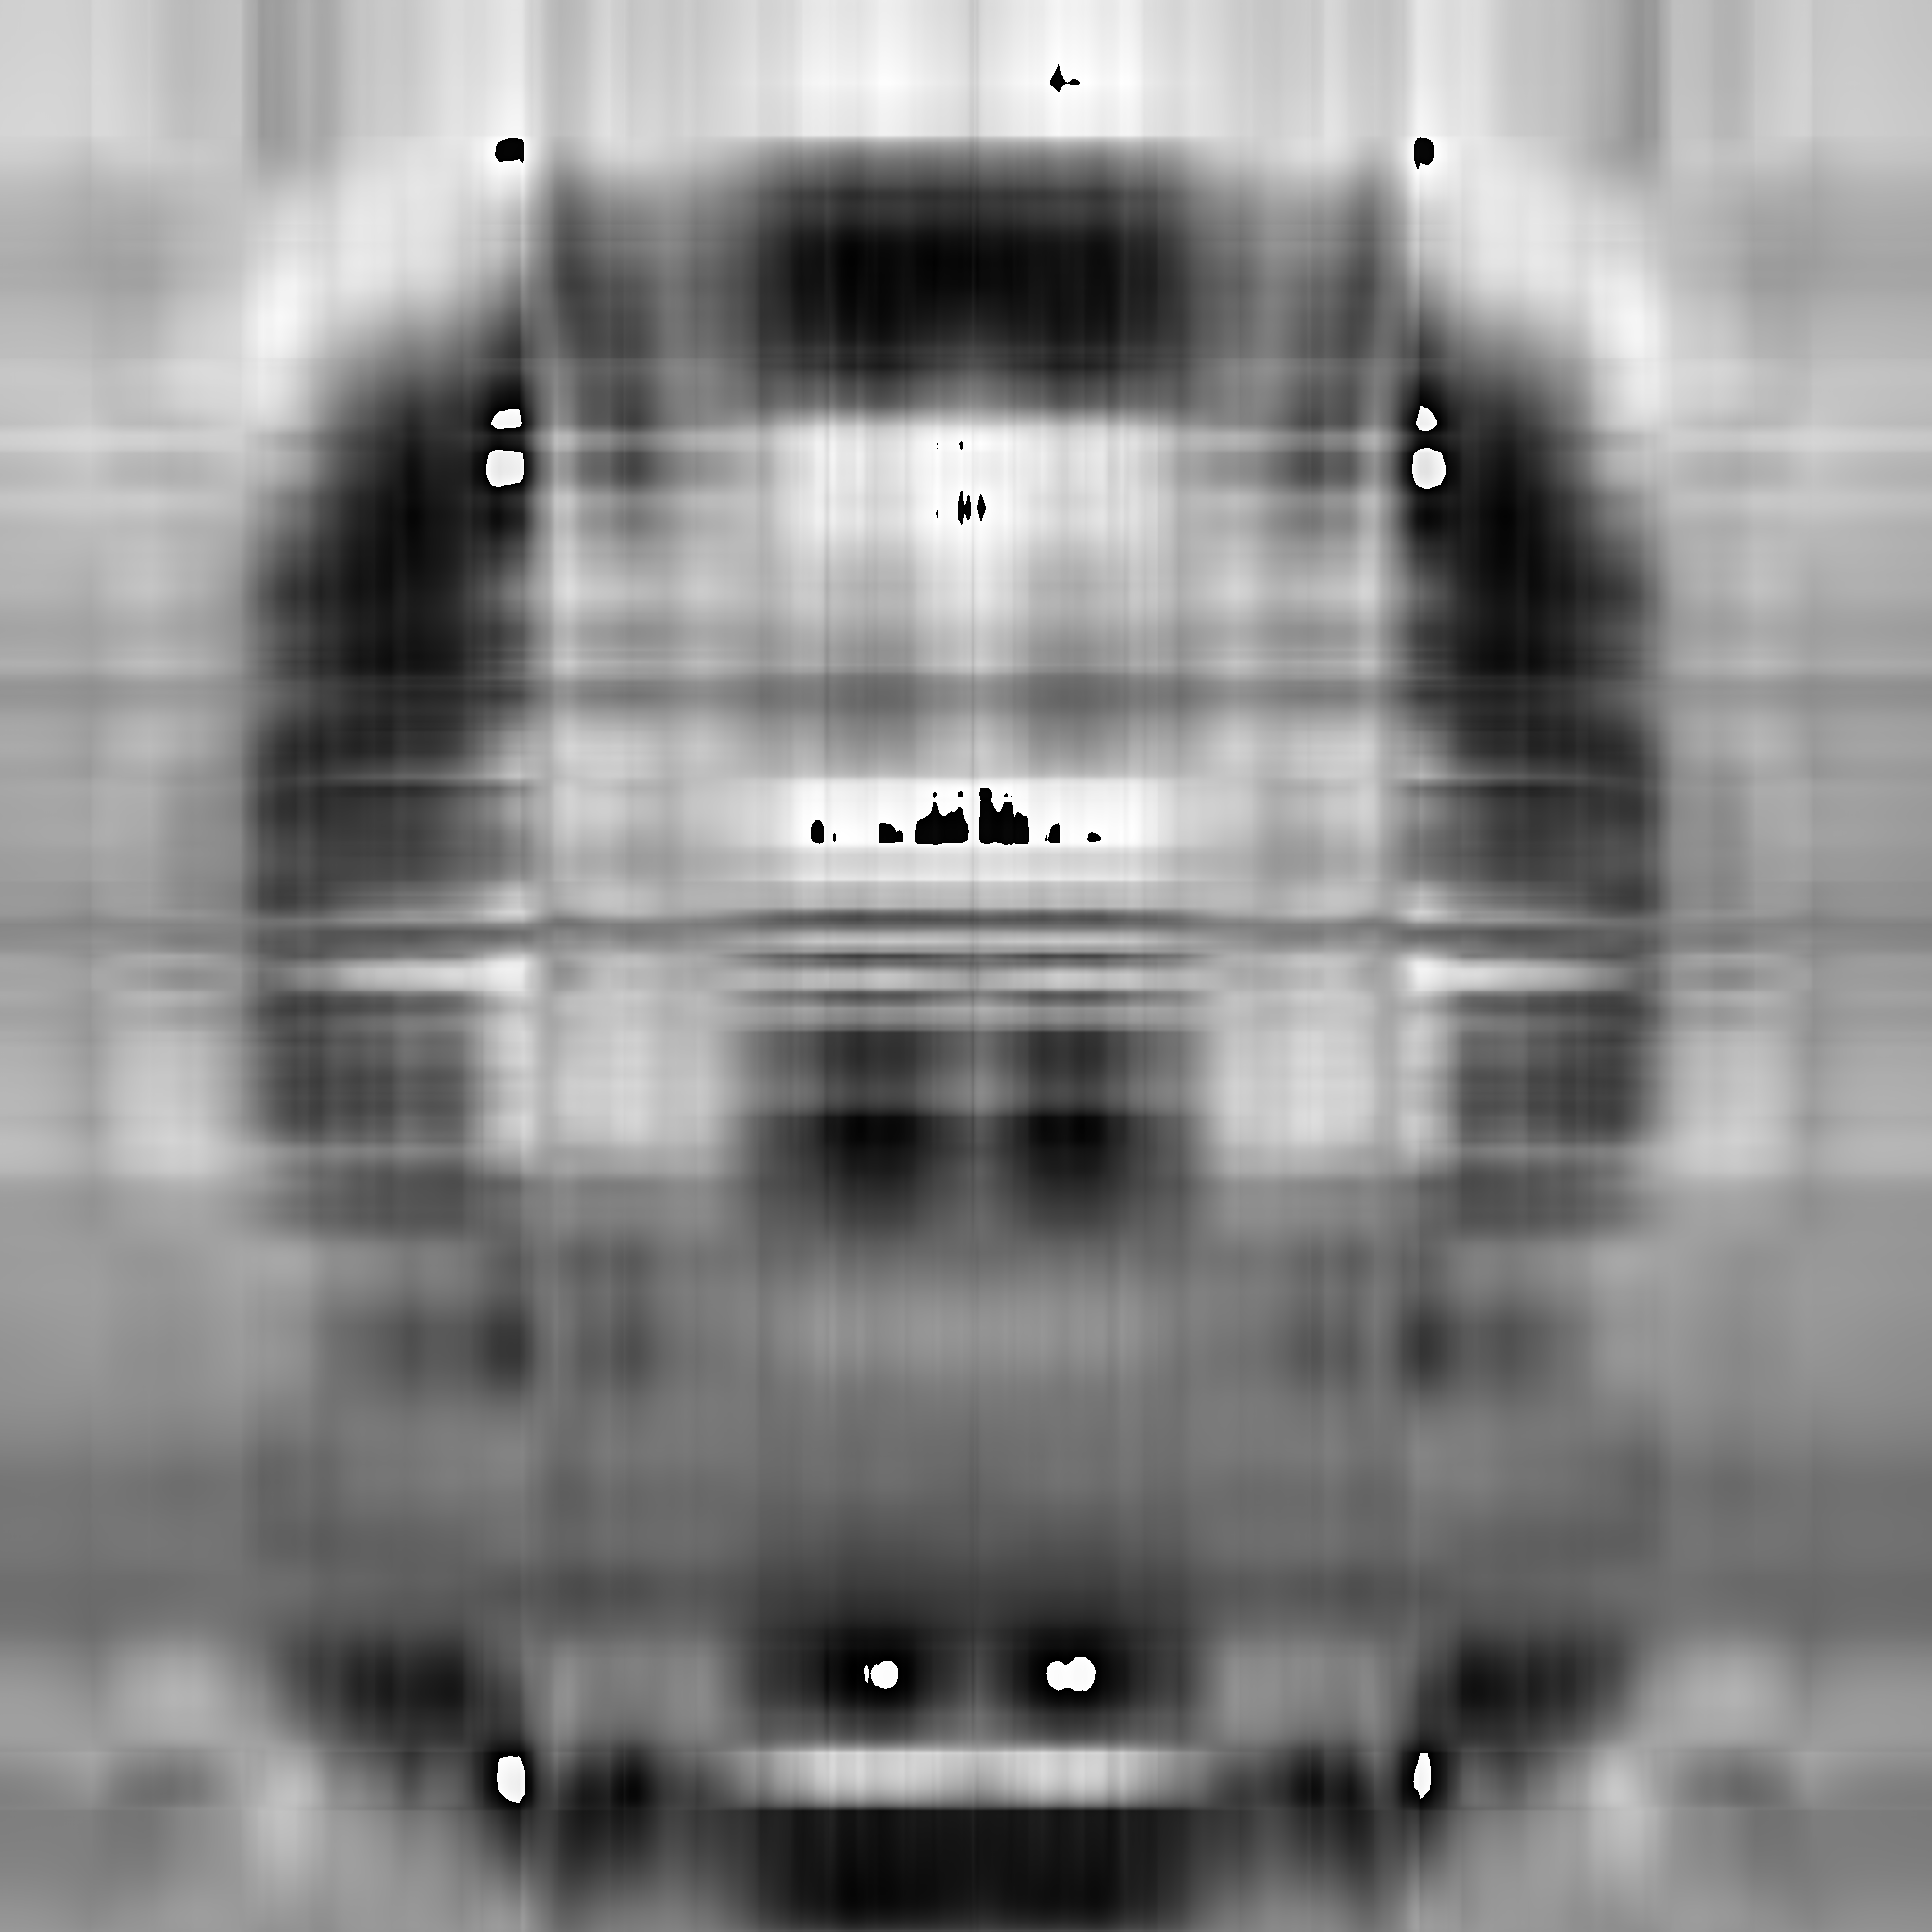
\includegraphics[width=\linewidth]{../image-compression/cat-4.png}
  \caption{$rank=4$}
  \label{fig:cat-bw-rank-4}
\end{figure}

\begin{figure}
  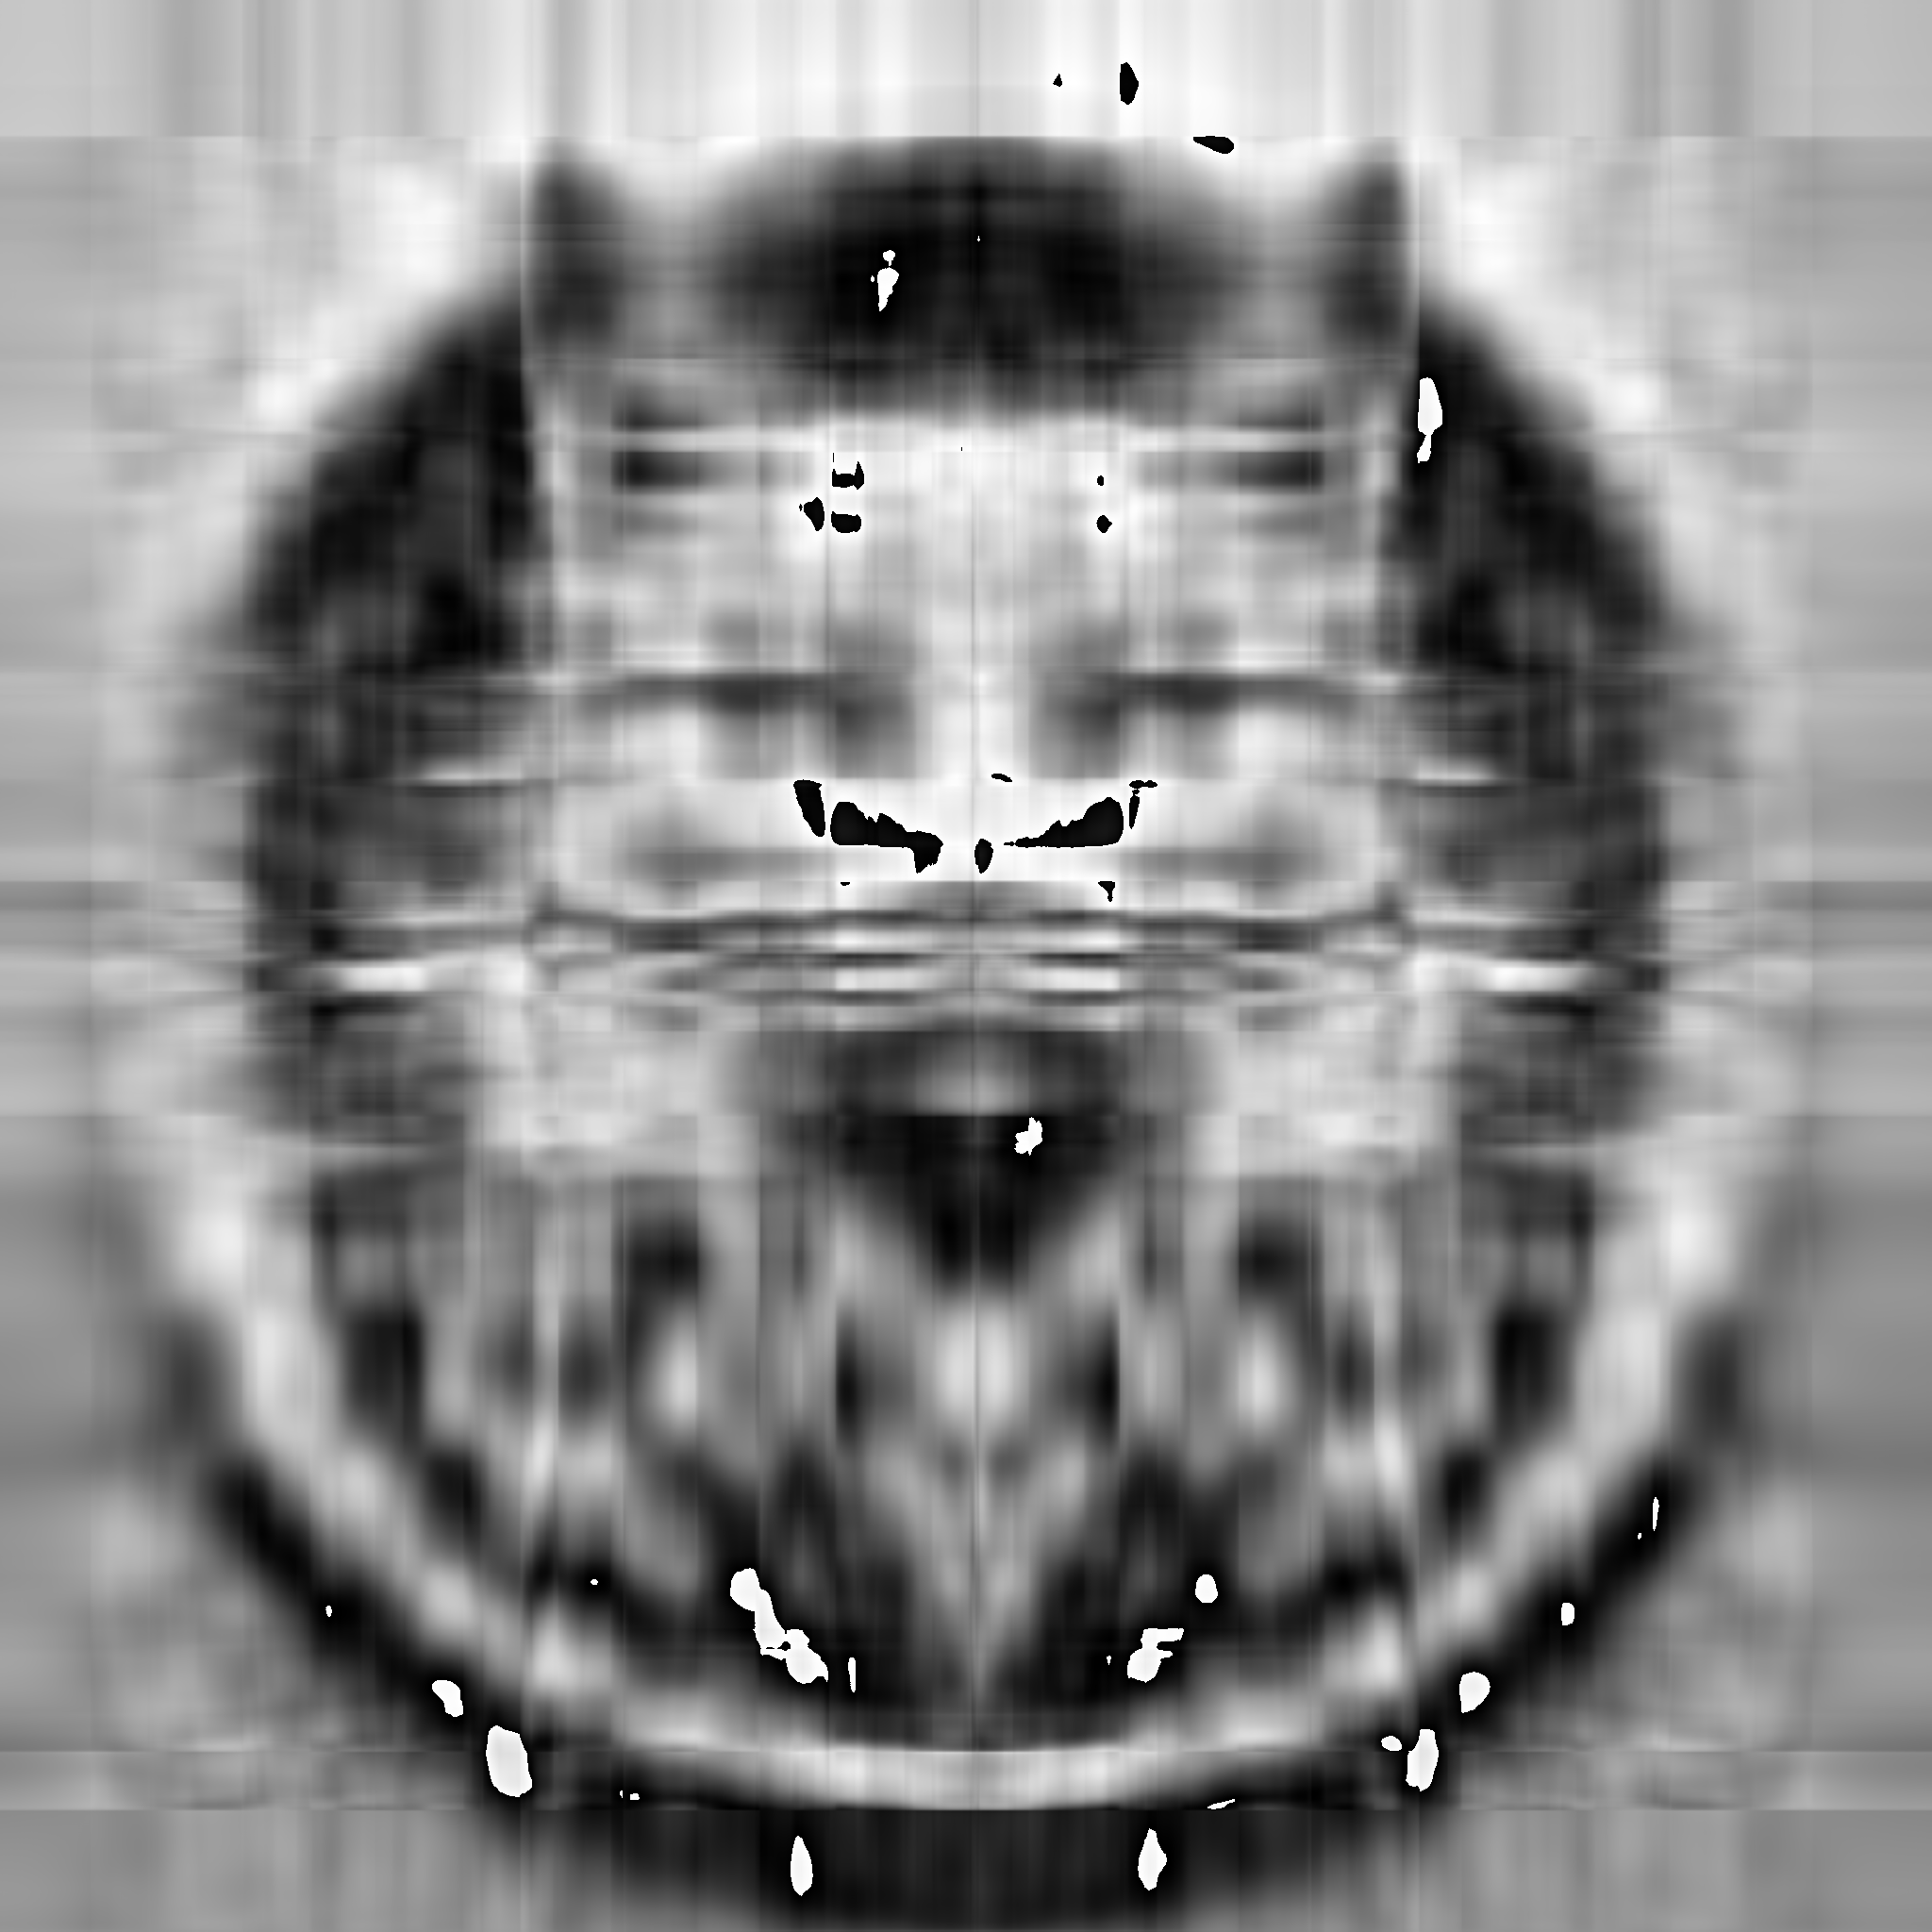
\includegraphics[width=\linewidth]{../image-compression/cat-8.png}
  \caption{$rank=8$}
  \label{fig:cat-bw-rank-8}
\end{figure}

\begin{figure}
  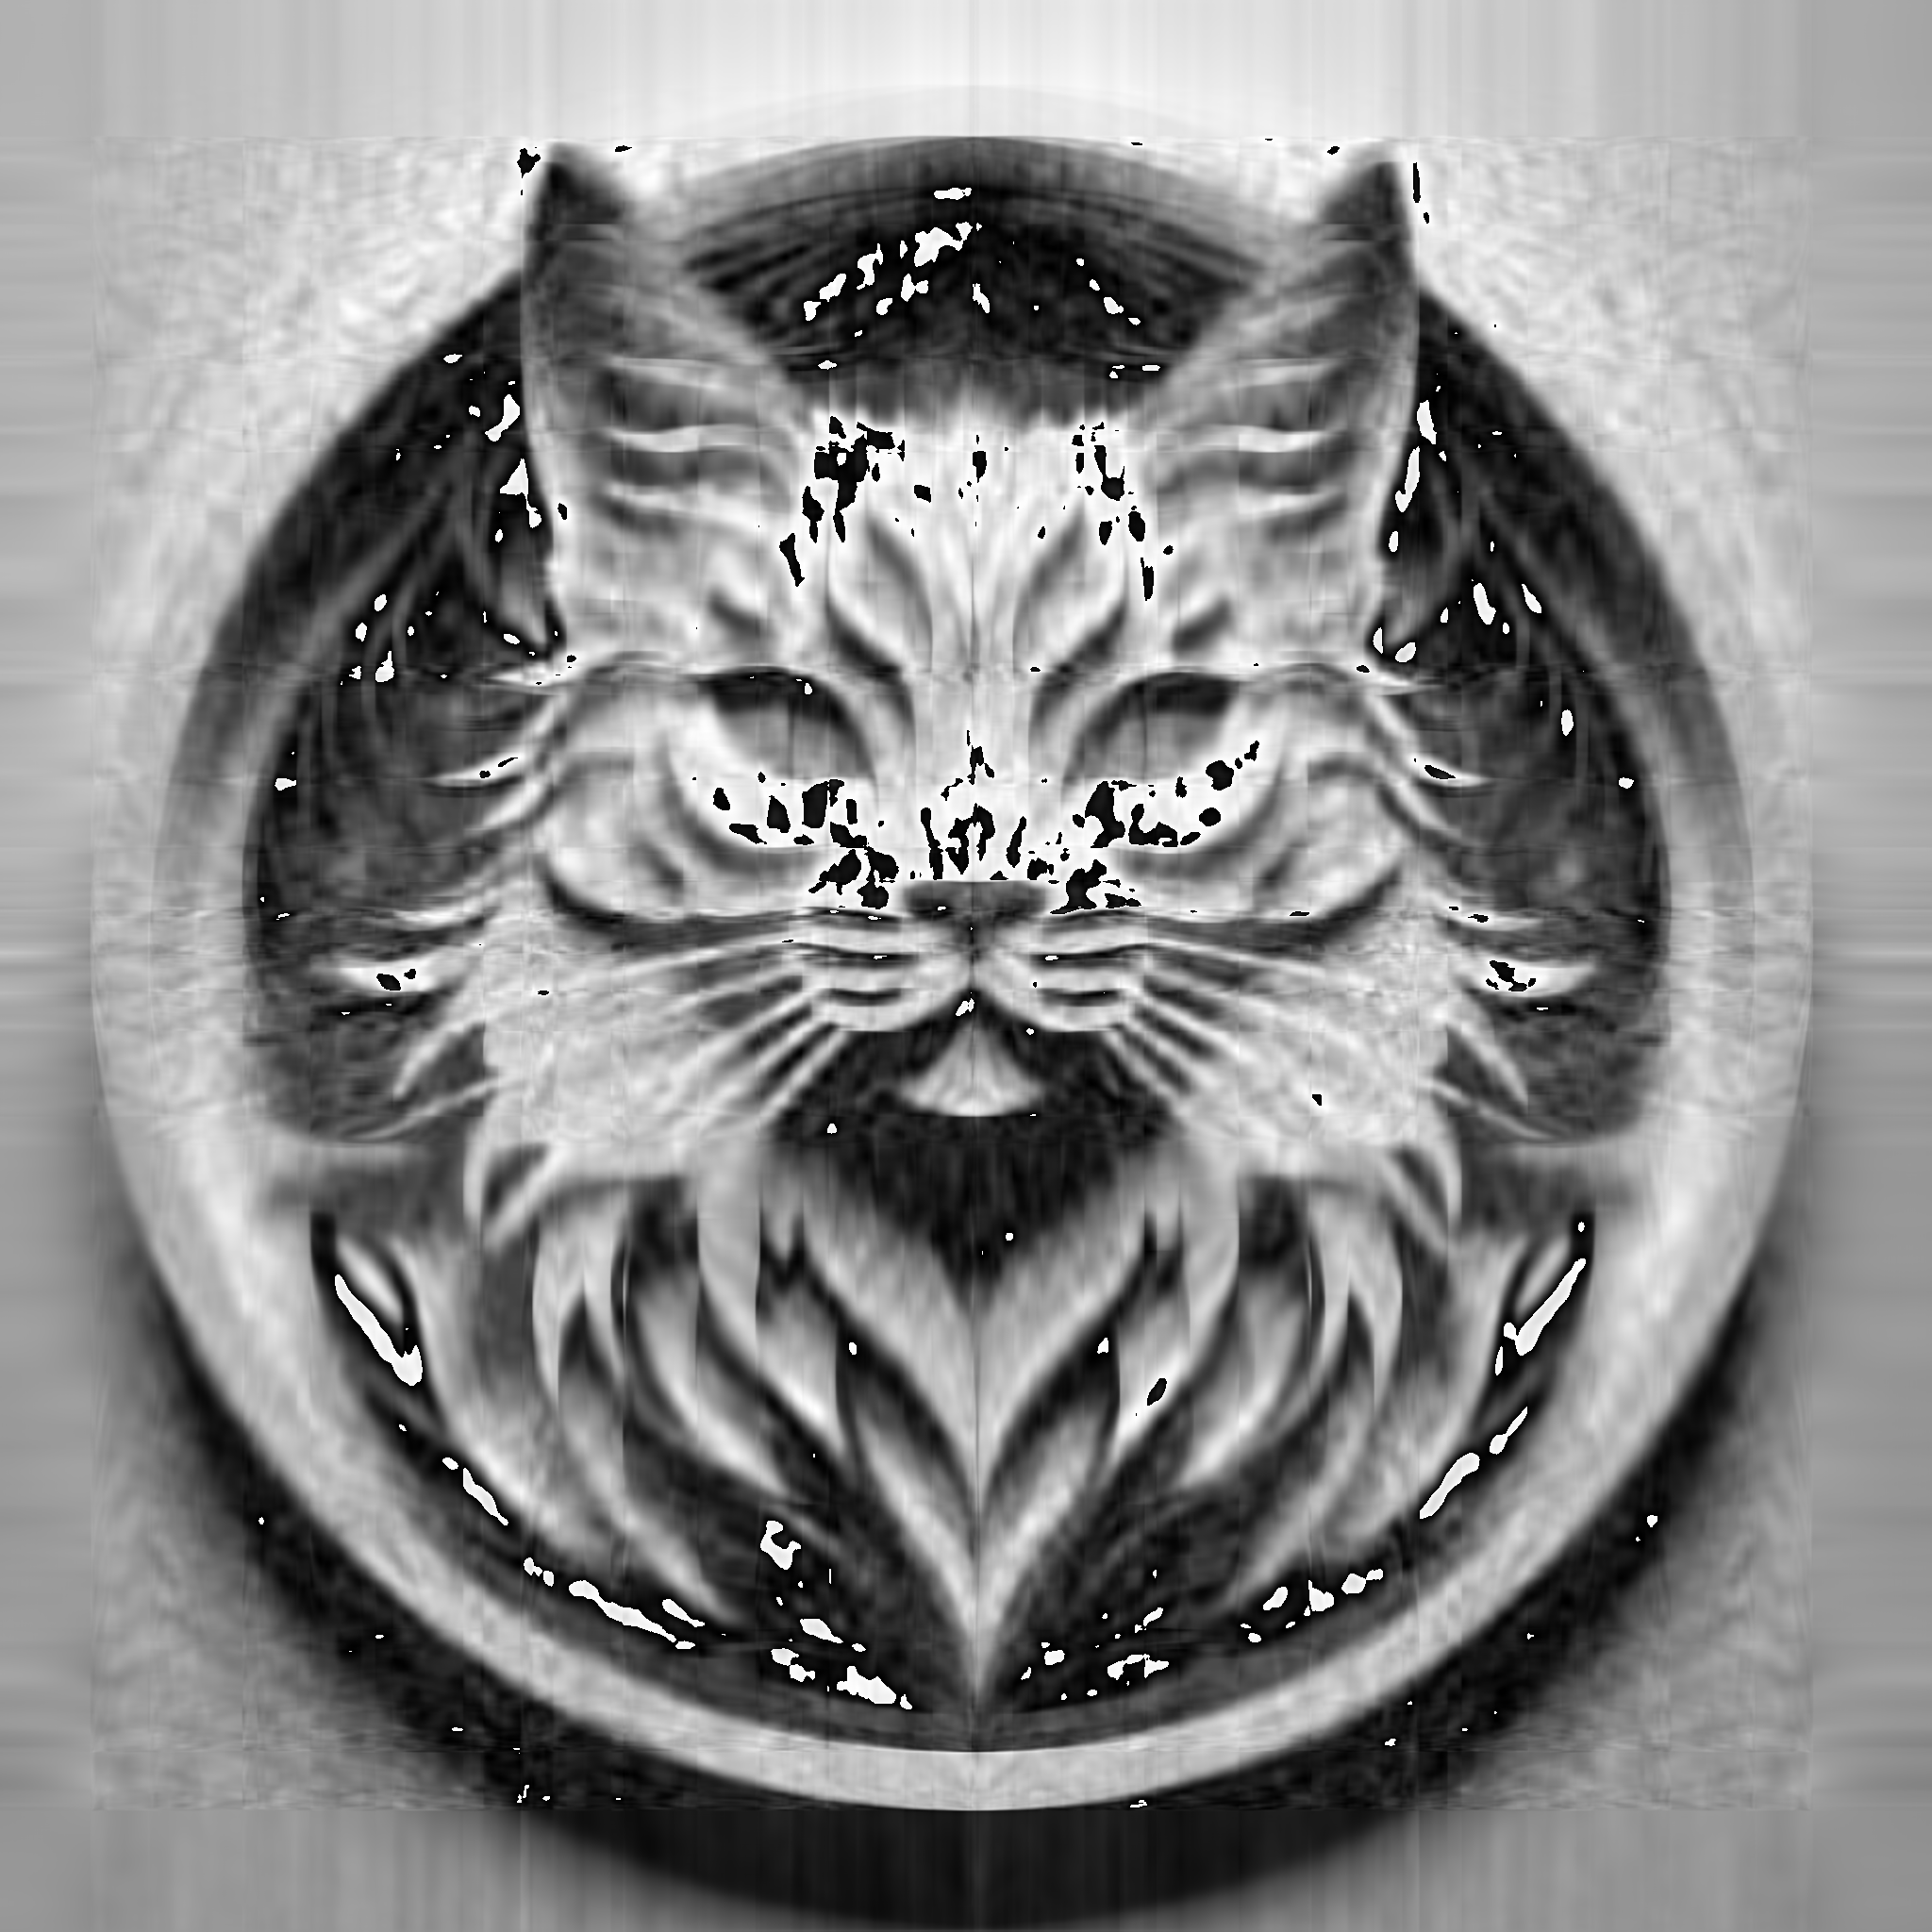
\includegraphics[width=\linewidth]{../image-compression/cat-32.png}
  \caption{$rank=32$}
  \label{fig:cat-bw-rank-32}
\end{figure}


\begin{figure}
  \includegraphics[width=\linewidth]{../image-compression/cat-256.png}
  \caption{$rank=256$}
  \label{fig:cat-bw-rank-256}
\end{figure}


\begin{figure}
  
\includegraphics[width=\linewidth]{../image-compression/cat-1024.png}
  \caption{$rank=1024$}
  \label{fig:cat-bw-rank-1024}
\end{figure}

\begin{figure}
  
\includegraphics[width=\linewidth]{../image-compression/cat-2048.png}
  \caption{$rank=2048$}
  \label{fig:cat-bw-rank-2048}
\end{figure}

همانطور که مشاهده می‌کنید، حتی در $rank$
پایین، کلیتی از تصویر دیده می‌شود، و با نزدیک شدن به سایز اصلی تصویر، تفاوت تقریبا ناچیز می‌باشد.

\subsection{بررسی خطا روش}
برای بررسی خطا در این روش
از دو معیار
\lr{MSE}
و
\lr{PSNR}
استفاده می‌کنیم.
\cite{4426357}
\cite{imcprichdavad}


برای محاسبه‌
$MSE$
یا
\lr{Mean Squared Error}
کافیست تفاوت تصویر نهایی به تصویر اولیه را محاسبه، و سپس مربعات ماتریس را میانگین بگیریم:

\begin{latin}
  \begin{python}
mse = np.mean((image - bw_image_array) ** 2)
  \end{python}
\end{latin}


معیار
$PSNR$
نشان دهنده‌ی میزان نویز به دیتا در تصویر می‌باشد.
روش حاسبه‌ی
$PSNR$
به شکل زیر می‌باشد:

\begin{equation}
  PSNR = 10 \log{10} \frac{255}{MSE}
\end{equation}


\begin{latin}
  \begin{python}
    psnr = 10 * (np.log10(255 / np.sqrt(mse)))
  \end{python}
\end{latin}


حال می‌توانیم این مقادیر را برای تقریب‌های مختلف محاسبه کرده و رسم کنیم:

\begin{latin}
  \begin{python}
from PIL import Image
import matplotlib.pyplot as plt
import matplotlib
import numpy as np
import os

image_name = "cat"
image_path = "./cat.png"

image = Image.open(image_path)

# Convert the image to grayscale (black and white)
bw_image = image.convert('L')
bw_image_array = np.array(bw_image)

U, S, VT = np.linalg.svd(bw_image_array)


def compress_image(U, S, Vt, rank):
    return U[:, :rank] @ np.diag(S[:rank]) @ Vt[:rank]


compression_ratios = [1, 4, 8, 16, 32, 64, 128, 256, 512, 750, 1000, 1024, 2048]

mse_values = []
psnr_values = []

for rank in compression_ratios:
    print("Rank", rank)
    image = compress_image(U, S, VT, rank)

    mse = np.mean((image - bw_image_array) ** 2)
    psnr = 10 * (np.log10(255 / np.sqrt(mse)))
    mse_values.append(mse)
    psnr_values.append(psnr)

plt.figure(figsize=(8, 6))
plt.plot(compression_ratios, mse_values, marker='o', color='blue', linestyle='-', linewidth=2, markersize=8)
plt.title('Mean Squared Error (MSE) vs. SVD compresssion')
plt.xlabel('Rank')
plt.ylabel('MSE')
plt.grid(True)
plt.tight_layout()
plt.savefig(os.path.join("../output", "image-comp-col-mse.jpg"))
matplotlib.rcParams.update({
    "pgf.texsystem": "xelatex",
    'text.usetex': True,
    'pgf.rcfonts': False,
    "font.family": "mononoki Nerd Font Mono",
    "font.serif": [],
    #  "font.cursive": ["mononoki Nerd Font", "mononoki Nerd Font Mono"],
})
plt.savefig(os.path.join("../output", "image-comp-col-mse.pgf"))
plt.show()

plt.figure(figsize=(8, 6))
plt.semilogx(compression_ratios, mse_values, marker='o', color='blue', linestyle='-', linewidth=2, markersize=8)
plt.title('Mean Squared Error (MSE) vs. log SVD compresssion')
plt.xlabel('Rank')
plt.ylabel('MSE')
plt.grid(True)
plt.tight_layout()
plt.savefig(os.path.join("../output", "image-comp-col-mse-log.jpg"))
matplotlib.rcParams.update({
    "pgf.texsystem": "xelatex",
    'text.usetex': True,
    'pgf.rcfonts': False,
    "font.family": "mononoki Nerd Font Mono",
    "font.serif": [],
    #  "font.cursive": ["mononoki Nerd Font", "mononoki Nerd Font Mono"],
})
plt.savefig(os.path.join("../output", "image-comp-col-mse-log.pgf"))
plt.show()

plt.figure(figsize=(8, 6))
plt.plot(compression_ratios, mse_values, marker='o', color='blue', linestyle='-', linewidth=2, markersize=8)
plt.title('PSNR vs. SVD compresssion')
plt.xlabel('Rank')
plt.ylabel('PSRN')
plt.grid(True)
plt.tight_layout()
plt.savefig(os.path.join("../output", "image-comp-psnr.jpg"))
matplotlib.rcParams.update({
    "pgf.texsystem": "xelatex",
    'text.usetex': True,
    'pgf.rcfonts': False,
    "font.family": "mononoki Nerd Font Mono",
    "font.serif": [],
    #  "font.cursive": ["mononoki Nerd Font", "mononoki Nerd Font Mono"],
})
plt.savefig(os.path.join("../output", "image-comp-col-psnr.pgf"))
plt.show()


plt.figure(figsize=(8, 6))
plt.semilogx(compression_ratios, mse_values, marker='o', color='blue', linestyle='-', linewidth=2, markersize=8)
plt.title('PSNR vs. log SVD compresssion')
plt.xlabel('Rank')
plt.ylabel('PSRN')
plt.grid(True)
plt.tight_layout()
plt.savefig(os.path.join("../output", "image-comp-col-psnr-log.jpg"))
matplotlib.rcParams.update({
    "pgf.texsystem": "xelatex",
    'text.usetex': True,
    'pgf.rcfonts': False,
    "font.family": "mononoki Nerd Font Mono",
    "font.serif": [],
    #  "font.cursive": ["mononoki Nerd Font", "mononoki Nerd Font Mono"],
})
plt.savefig(os.path.join("../output", "image-comp-col-psnr-log.pgf"))
plt.show()

  \end{python}
\end{latin}


\insertfig{../output/image-comp-mse.pgf}{\lr{MSE vs Rank}}{bw_comp_mse}
\insertfig{../output/image-comp-mse-log.pgf}{\lr{MSE vs log Rank}}{bw_comp_mse_log}
\insertfig{../output/image-comp-psnr.pgf}{\lr{PSNR vs Rank}}{bw_comp_psnr}
\insertfig{../output/image-comp-psnr-log.pgf}{\lr{PSNR vs log Rank}}{bw_comp_psnr_log}

همانطور که مشاهده میشود، بخش عمده بهینه سازی تا
$rank=256$
انجام میشود که حدود
$12.5\%$
ابعاد اصلی تصویر می‌باشد.


\subsection{پیاده سازی با تصاویر رنگی}
هر تصویر رنگی، شامل سه بخش
\lr{R, G, B}
می‌باشد که هریک نمایانگر میزان یکی از رنگ‌های قرمز، سبز،و آبی اند.
برای پیاده سازی این روش در یک تصویر رنگی، کافیست برای هر یک از
\lr{channel}
ها این پروسه‌را انجام دهیم، و سپس نتیجه هر سه را کنار یکدیگر قرار دهیم:



\begin{latin}
  \begin{python}
image_name = "cat"
image_path = "./cat.png"


from PIL import Image
import matplotlib.pyplot as plt
import numpy as np
import os

image = Image.open(image_path)

# Convert the image to grayscale (black and white)
bw_image_array = np.array(image)

plt.imshow(image_array)
plt.axis('off')
plt.show()

R_U, R_S, R_VT = np.linalg.svd(image_array[:, :, 0])
G_U, G_S, G_VT = np.linalg.svd(image_array[:, :, 1])
B_U, B_S, B_VT = np.linalg.svd(image_array[:, :, 2])

compression_ratios = [1, 4, 8, 16, 32, 64, 128, 256, 512, 750, 1000, 1024, 2048]
save_grayscale_image(bw_image_array, "cat-rgb.png")
original_size = os.path.getsize("cat-rgb.png")

rank_errors = []

for rank in compression_ratios:
    print("Rank", rank)
    image_R = compress_image(R_U, R_S, R_VT, rank)
    image_G = compress_image(G_U, G_S, G_VT, rank)
    image_B = compress_image(B_U, B_S, B_VT, rank)
    image = np.dstack((image_R, image_G, image_B))

    if image.dtype != np.uint8:
        image = image.astype(np.uint8)
    filename = f"cat-{rank}.png"
    save_image(image, filename)
    result_size = os.path.getsize(filename)
    print(f"Size {result_size / 1024 / 1024:.2}Mb", )
    show_image(image)

  \end{python}
\end{latin}


نتیجه برای تصاویر رنگی به این شکل خواهد بود:


\begin{figure}
  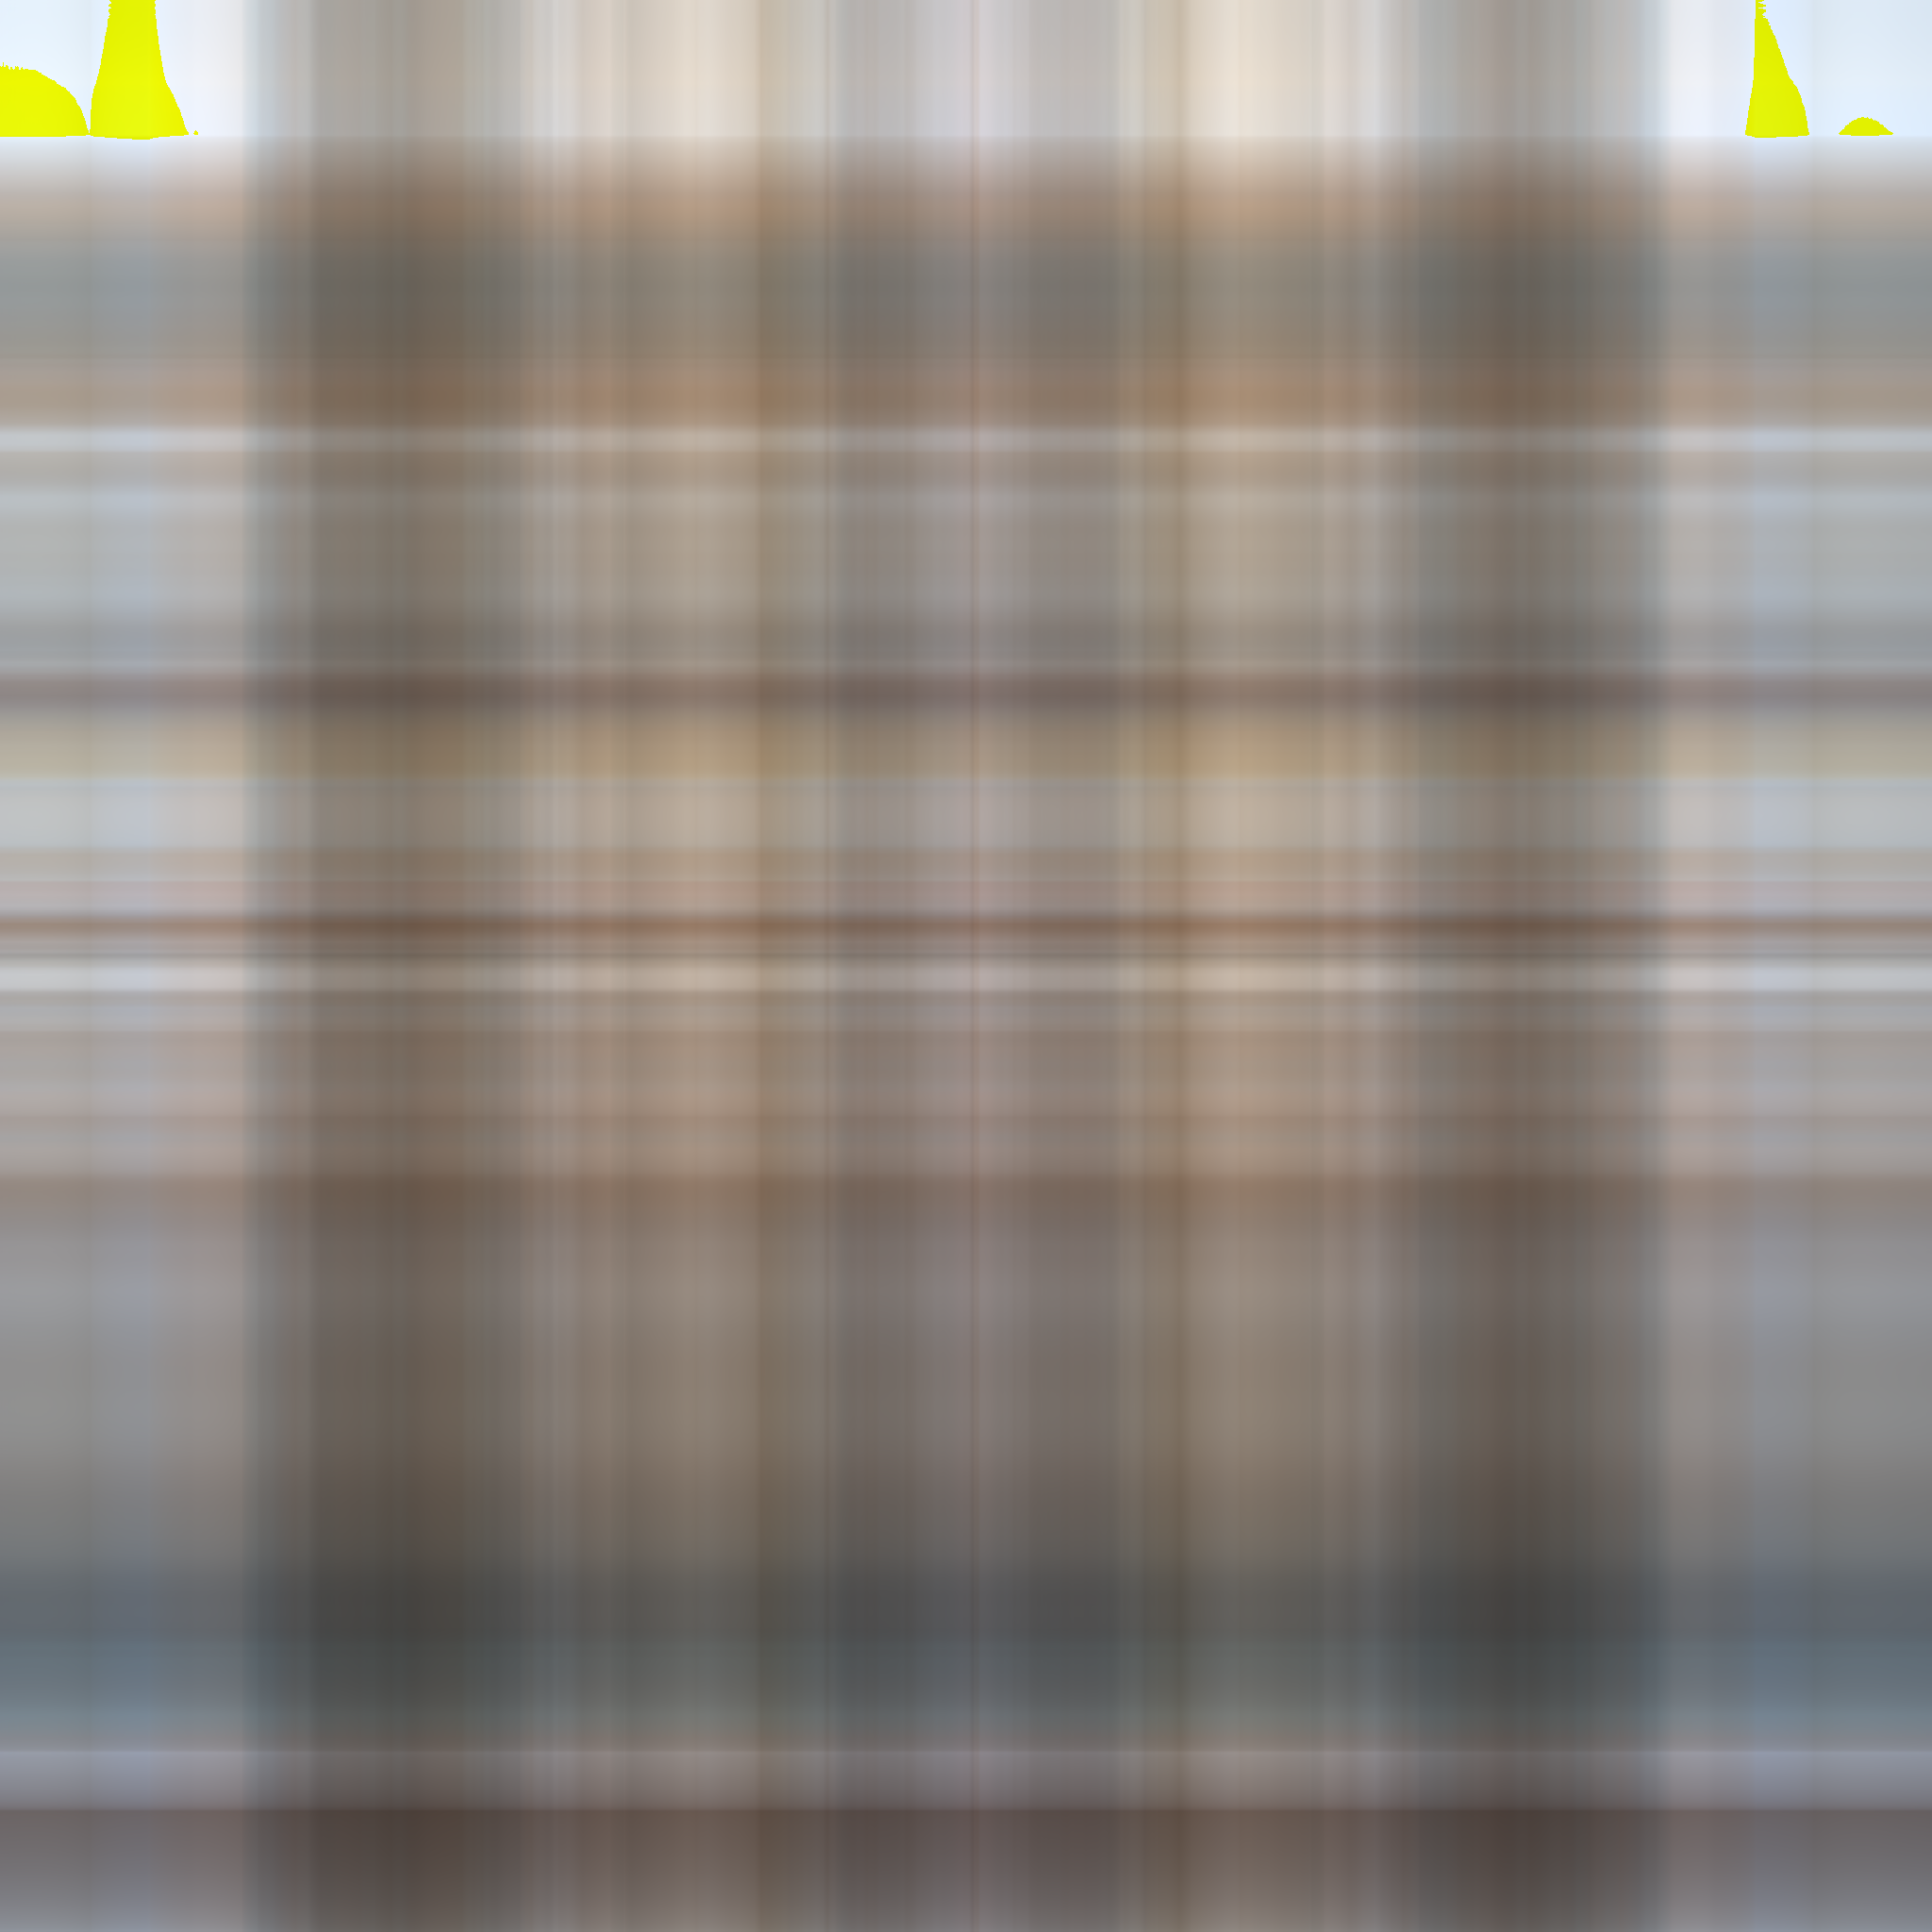
\includegraphics[width=\linewidth]{../image-compression-color/cat-1.png}
  \caption{$rank=1$}
  \label{fig:cat-bw-rank-1}
\end{figure}

\begin{figure}
  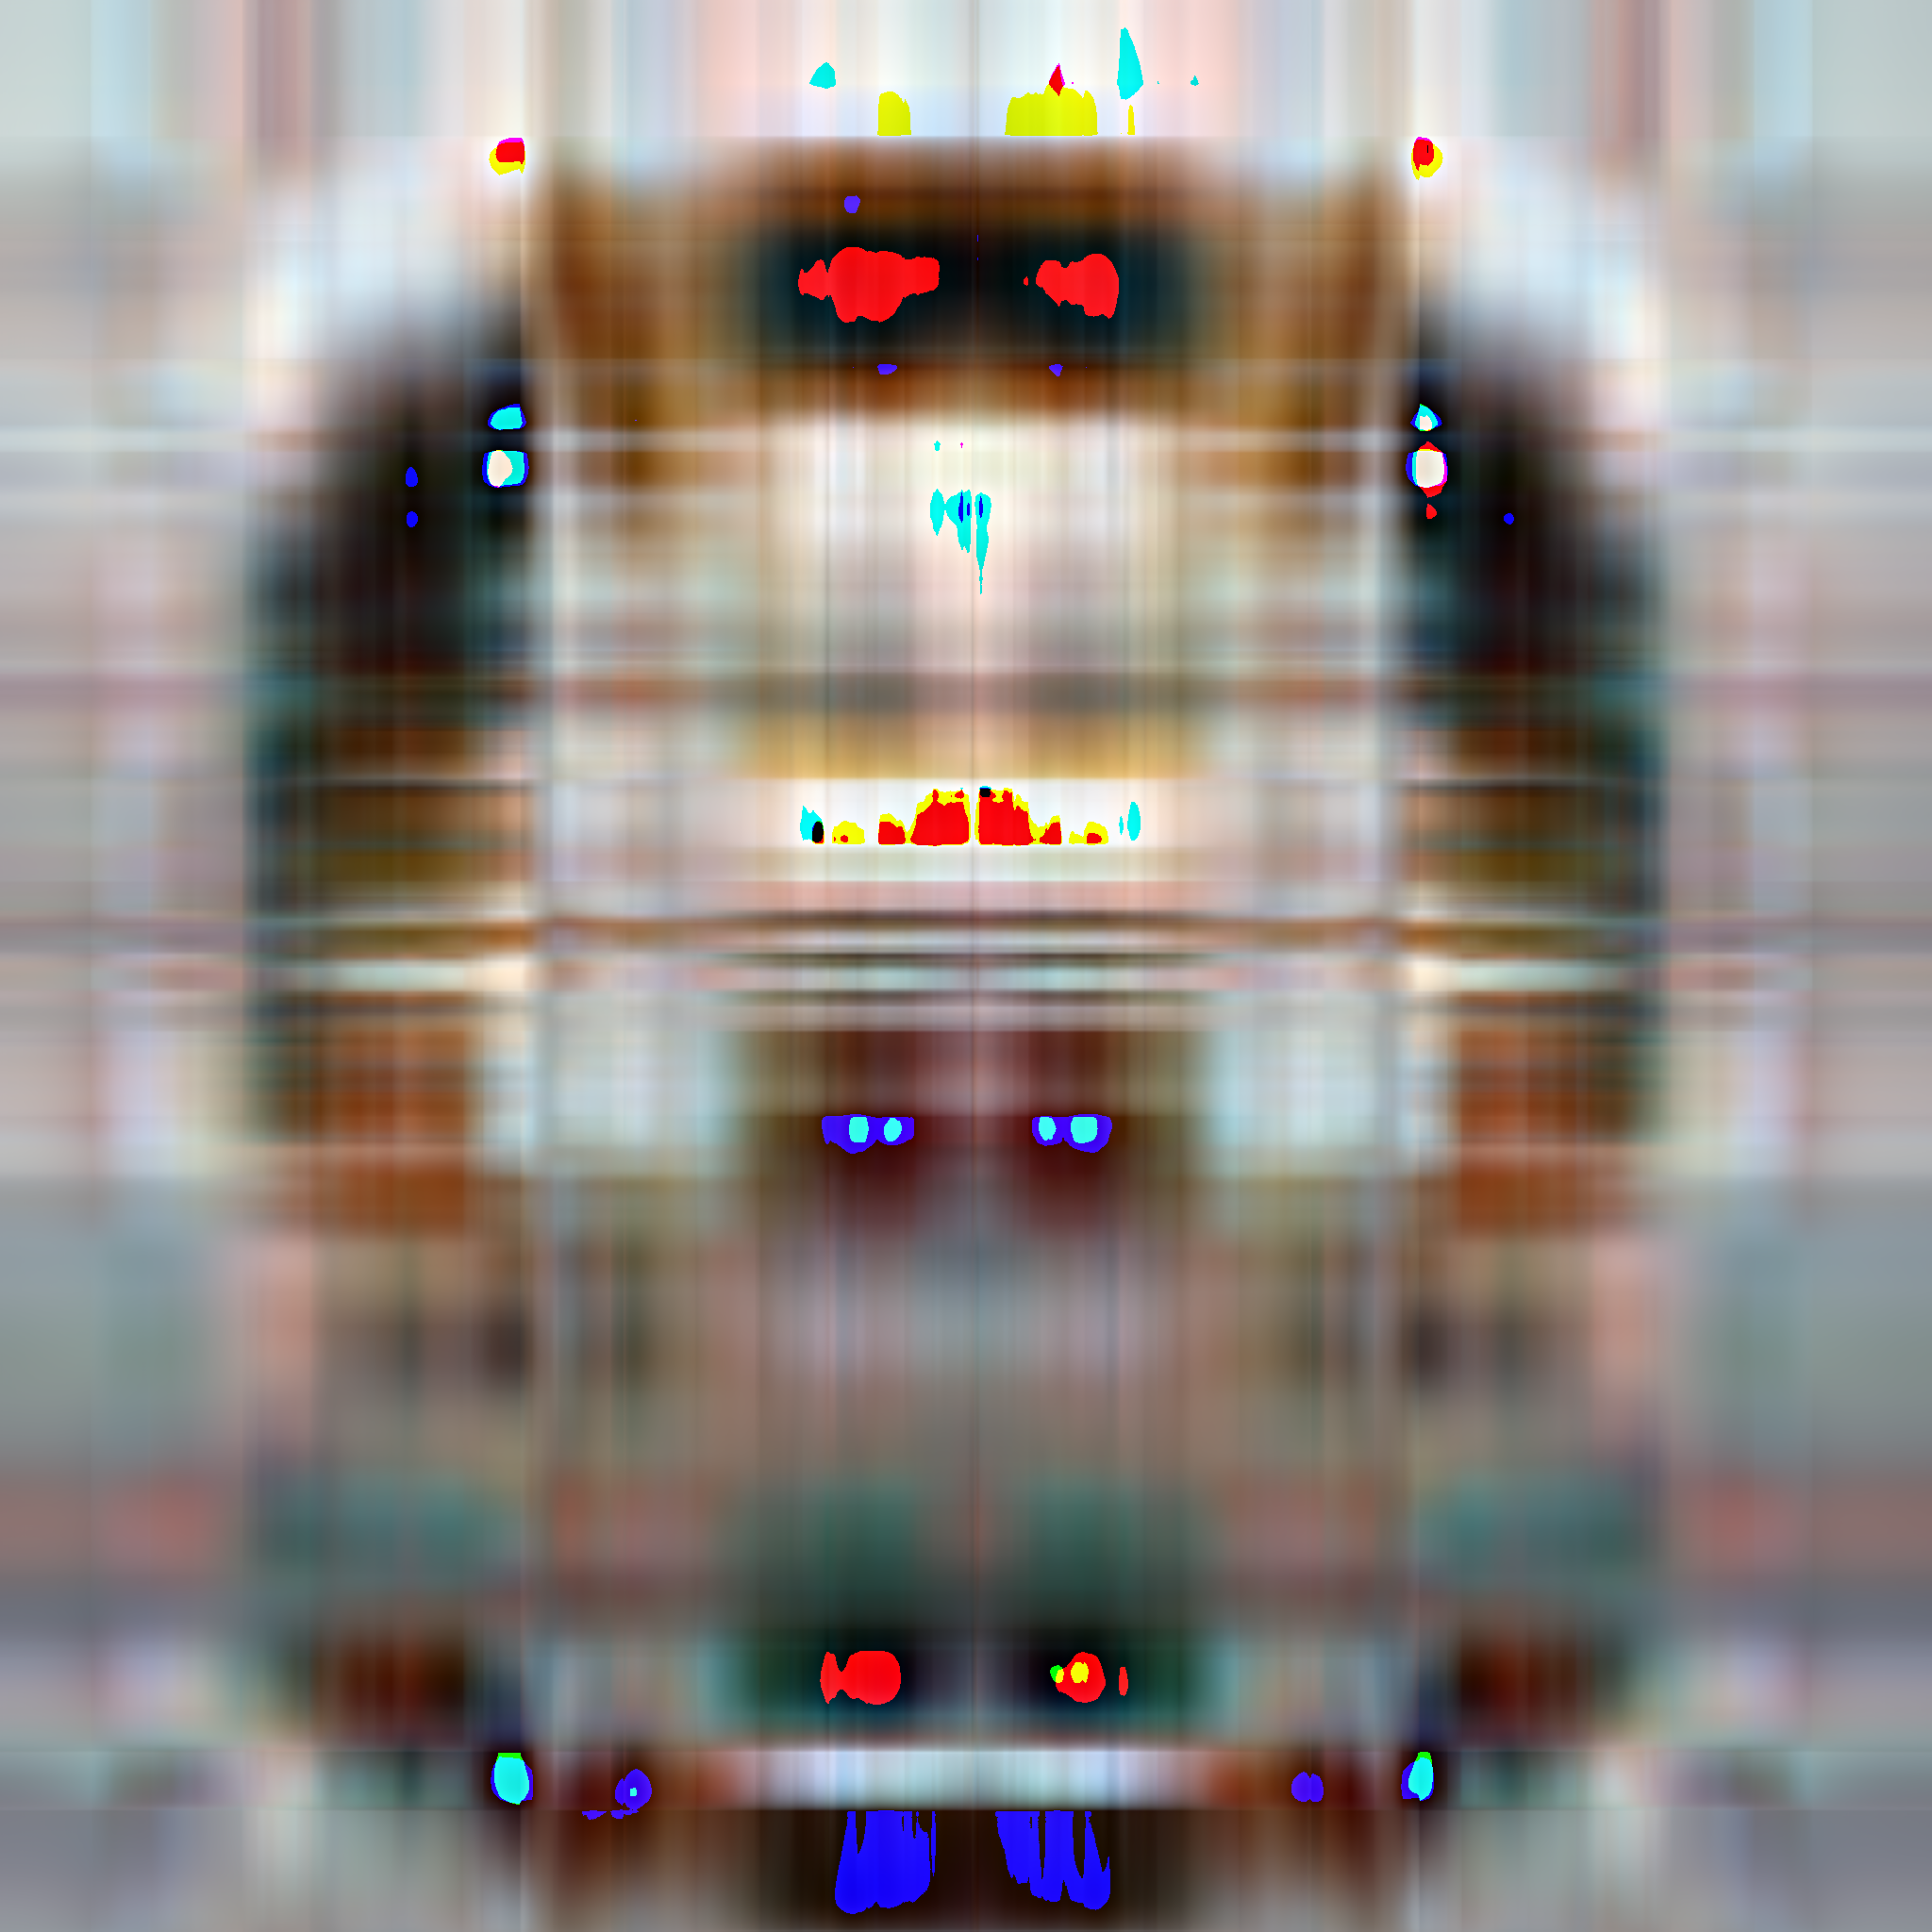
\includegraphics[width=\linewidth]{../image-compression-color/cat-4.png}
  \caption{$rank=4$}
  \label{fig:cat-bw-rank-4}
\end{figure}

\begin{figure}
  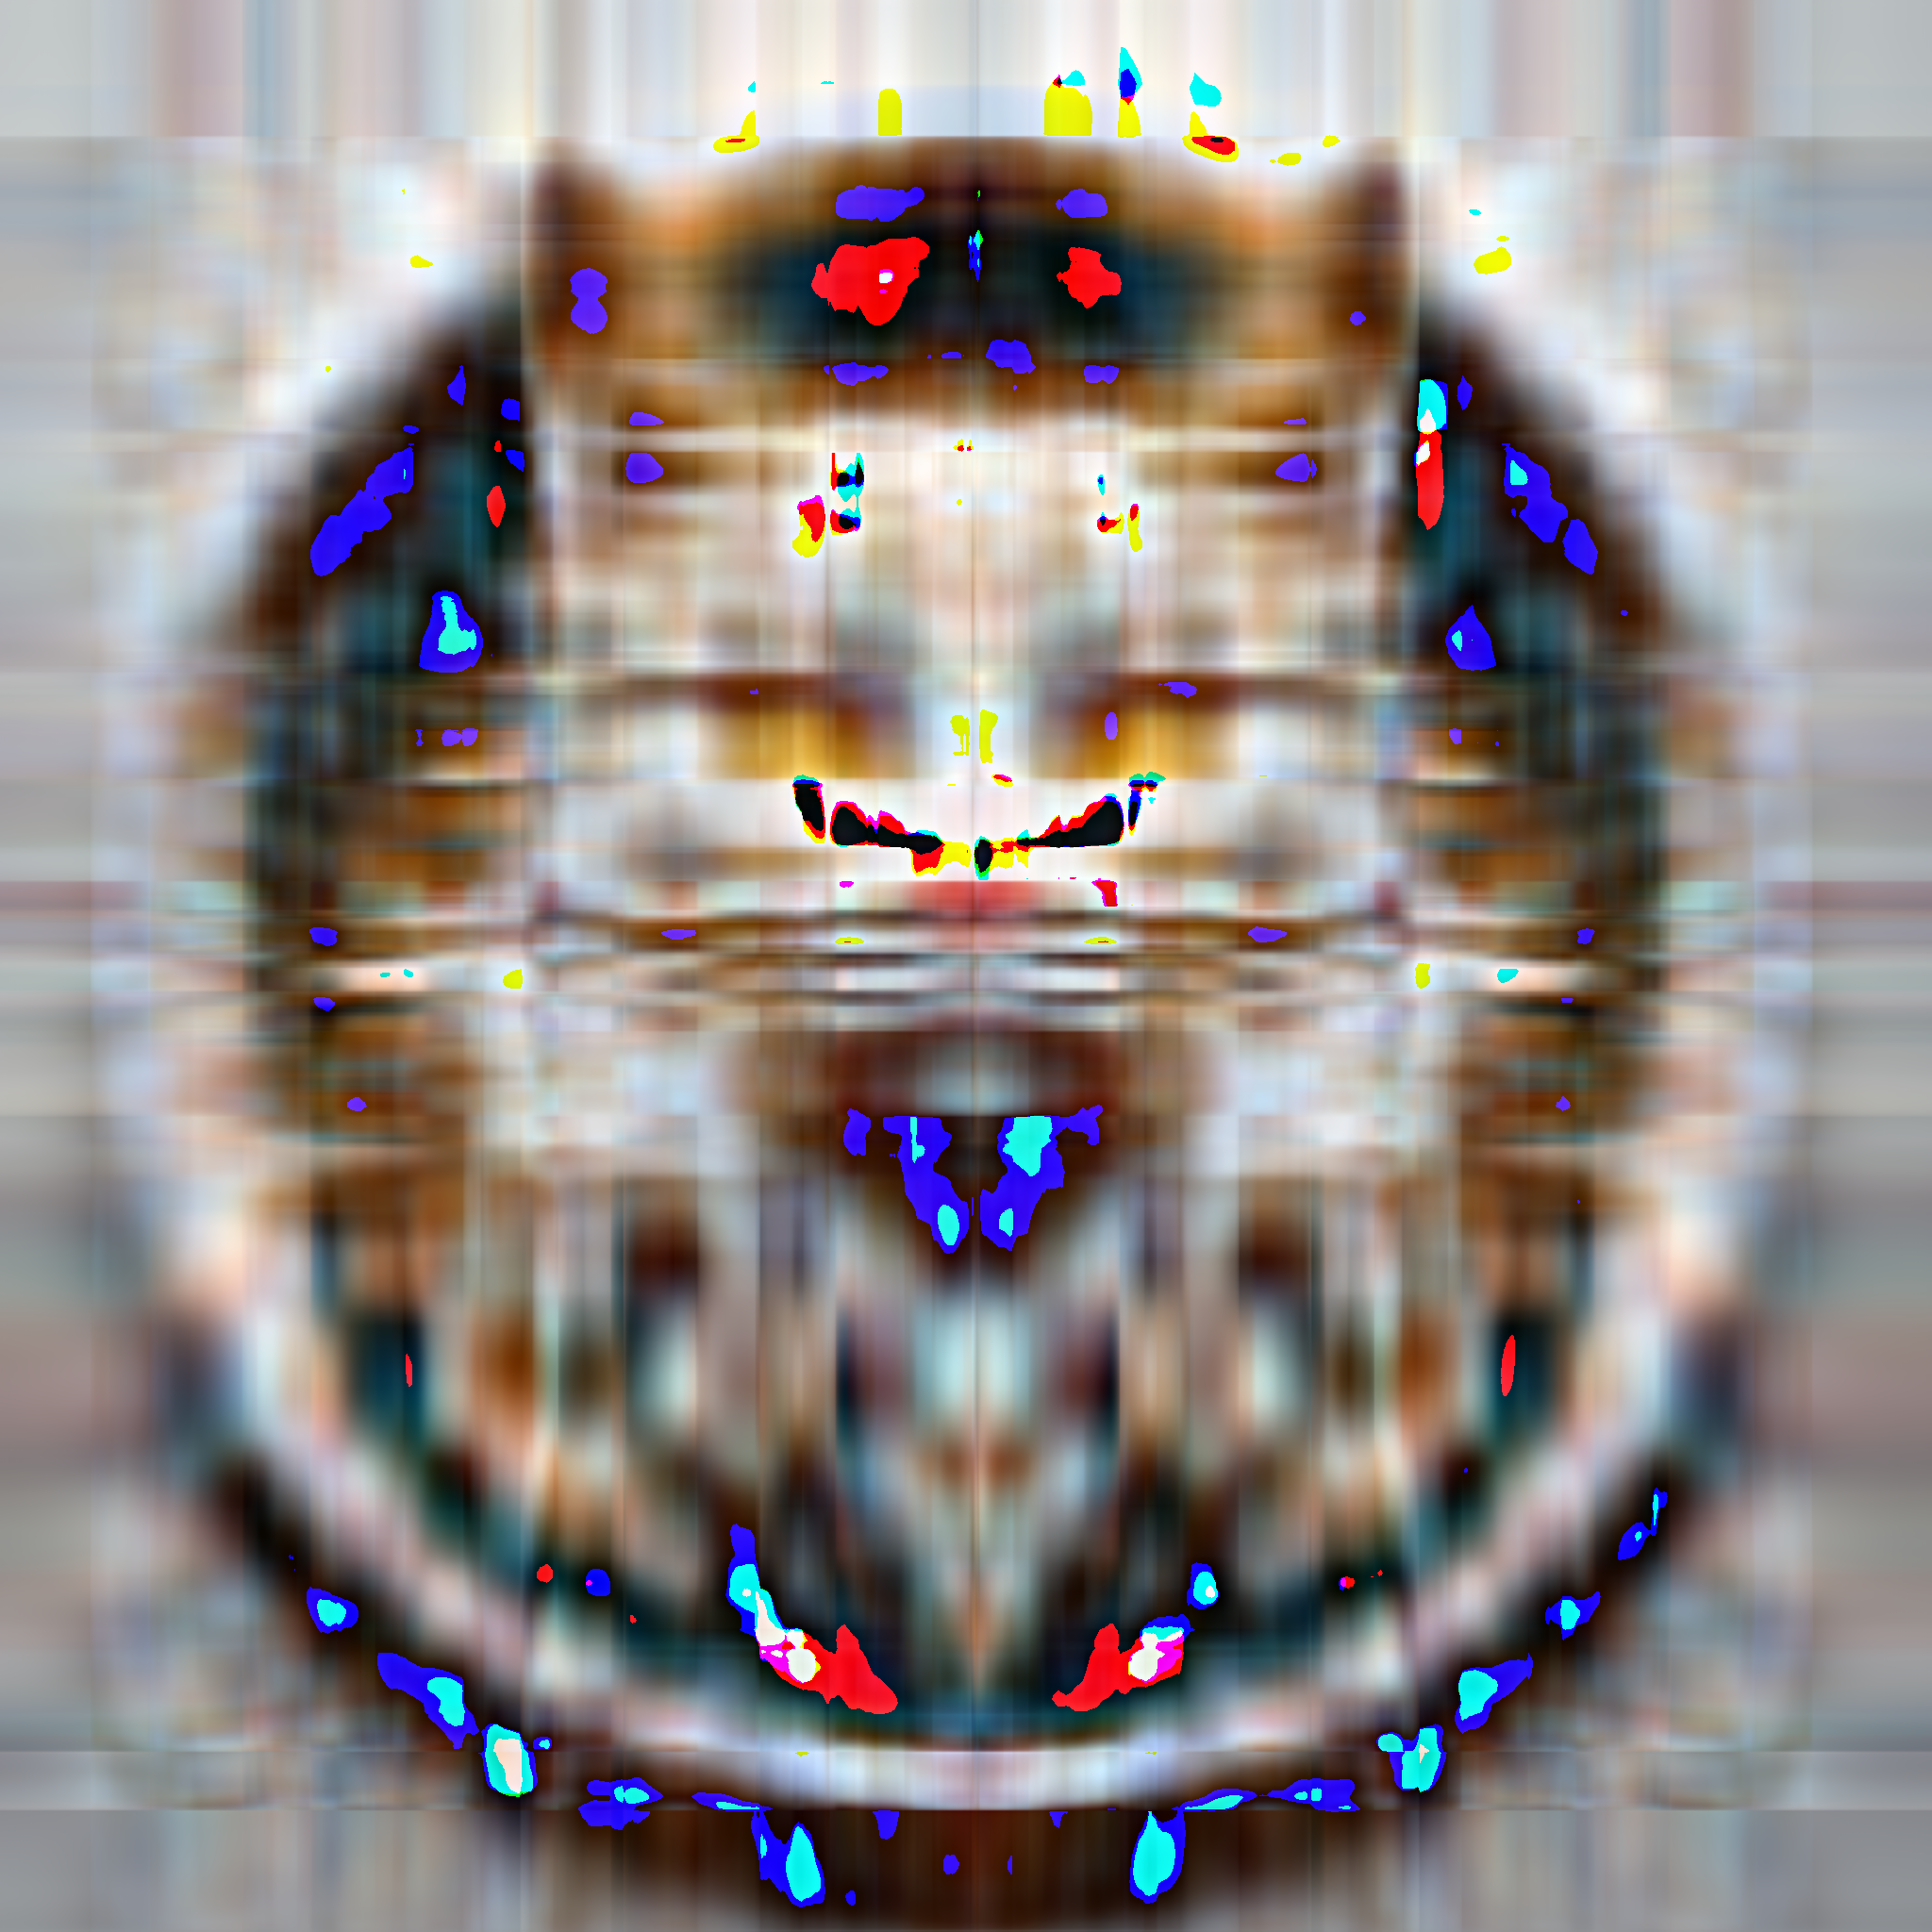
\includegraphics[width=\linewidth]{../image-compression-color/cat-8.png}
  \caption{$rank=8$}
  \label{fig:cat-bw-rank-8}
\end{figure}

\begin{figure}
  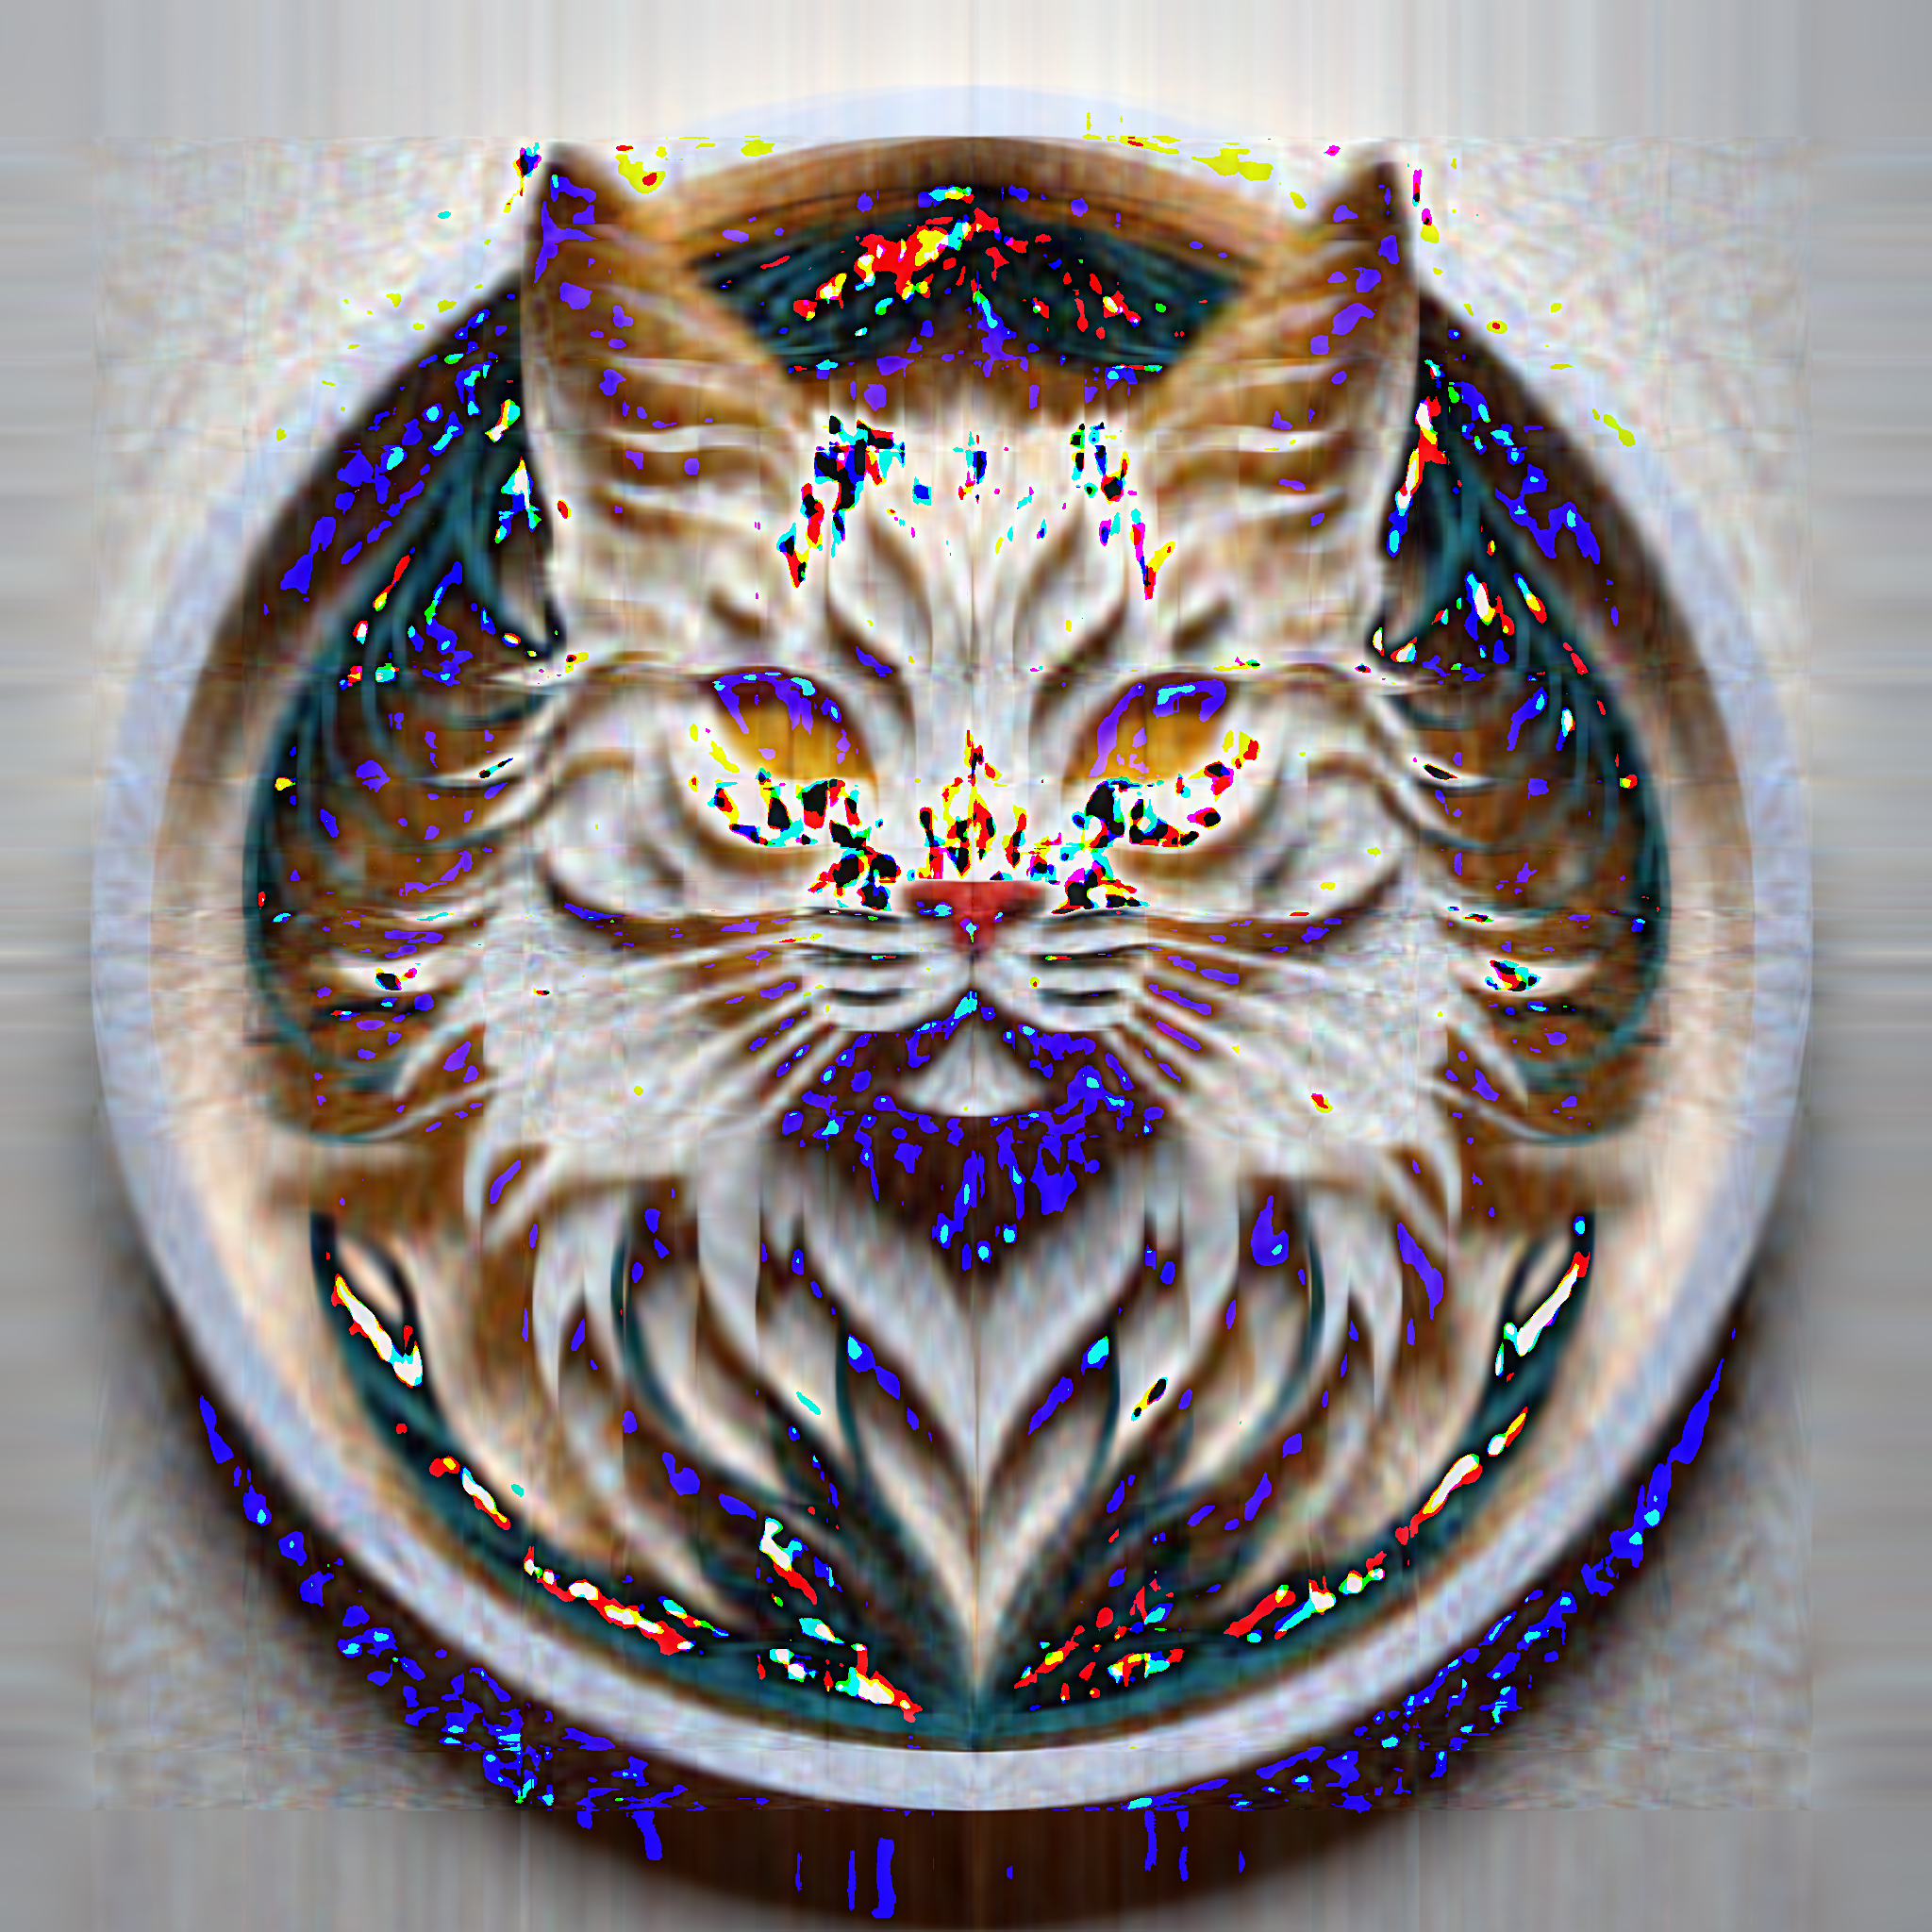
\includegraphics[width=\linewidth]{../image-compression-color/cat-32.png}
  \caption{$rank=32$}
  \label{fig:cat-bw-rank-32}
\end{figure}


\begin{figure}
  \includegraphics[width=\linewidth]{../image-compression-color/cat-256.png}
  \caption{$rank=256$}
  \label{fig:cat-bw-rank-256}
\end{figure}


\begin{figure}
  
\includegraphics[width=\linewidth]{../image-compression-color/cat-1024.png}
  \caption{$rank=1024$}
  \label{fig:cat-bw-rank-1024}
\end{figure}

\begin{figure}
  
\includegraphics[width=\linewidth]{../image-compression-color/cat-2048.png}
  \caption{$rank=2048$}
  \label{fig:cat-bw-rank-2048}
\end{figure}

\insertfig{../output/image-comp-col-mse.pgf}{\lr{MSE vs Rank}}{bw_comp_col_mse}
\insertfig{../output/image-comp-col-mse-log.pgf}{\lr{MSE vs log Rank}}{bw_comp_col_mse_log}
\insertfig{../output/image-comp-col-psnr.pgf}{\lr{PSNR vs Rank}}{bw_comp_col_psnr}
\insertfig{../output/image-comp-col-psnr-log.pgf}{\lr{PSNR vs log Rank}}{bw_comp_col_psnr_log}

\chapter{نتیجه گیری}
این روش برای به دست ‌آوردن تصاویر کم حجم مفید است، اما  نتیجه آن از دید انسانی مناسب نیست.
روش‌های دیگری که تمرکز روی نزدیکی نتایج از دید انسان دارند مانند روشی که برای کاهش حجم
\lr{jpg}
استفاده می‌شود
به مراتب نتایج بهتری نسبت به این روش ارائه می‌دهند.

%\include{chapter4}
%\include{chapter5}

%--------------------------------------------------------------------------appendix( مراجع و پیوست ها)
\chapterfont{\vspace*{-2em}\centering\LARGE}%

\appendix
\bibliographystyle{plain-fa}
\bibliography{references}
\chapter*{‌پیوست}
\markboth{پیوست}{}
\addcontentsline{toc}{chapter}{پیوست}
%--------------------------------------------------------------------------dictionary(واژه نامه ها)
%اگر مایل به داشتن صفحه واژه‌نامه نیستید، خط زیر را غیر فعال کنید.
%\parindent=0pt
%%
\chapter*{واژه‌نامه‌ی فارسی به انگلیسی}
\pagestyle{style9}

\addcontentsline{toc}{chapter}{واژه‌نامه‌ی فارسی به انگلیسی}
%%%%%%
\begin{multicols*}{2}

{\bf آ}
\vspace*{3mm}


\farsiTOenglish{اسکالر}{Scalar}


\vspace*{3mm}
{\bf ب}
\vspace*{3mm}

\farsiTOenglish{بالابر}{Lift}


\vspace*{3mm}
{\bf پ}
%%\vspace*{3mm}

\farsiTOenglish{پایا}{Invariant}



\vspace*{3mm}
{\bf ت}
%%\vspace*{3mm}

\farsiTOenglish{ تناظر }{Correspondence}


\vspace*{3mm}
{\bf ث}
%%\vspace*{3mm}

\farsiTOenglish{ثابت‌ساز}{Stabilizer}

\vspace*{3mm}
{\bf ج}
%%\vspace*{3mm}

\farsiTOenglish{جایگشت}{Permutation}



\vspace*{3mm}
{\bf چ}
%%\vspace*{3mm}


\farsiTOenglish{چند جمله‌ای }{Polynomial}

\vspace*{3mm}
{\bf ح}
%%\vspace*{3mm}

\farsiTOenglish{حاصل‌ضرب دکارتی}{Cartesian product}


\vspace*{3mm}
{\bf خ}
%%\vspace*{3mm}

\farsiTOenglish{خودریختی}{Automorphism}

\vspace*{3mm}
{\bf د}
%%\vspace*{3mm}

\farsiTOenglish{درجه}{Degree}


\vspace*{3mm}
{\bf ر}
%%\vspace*{3mm}


\farsiTOenglish{ریزپردازنده}{microprocessor}


\vspace*{3mm}
{\bf ز}
%%\vspace*{3mm}


\farsiTOenglish{زیرمدول}{Submodule}


\vspace*{3mm}
{\bf س}
%%\vspace*{3mm}

\farsiTOenglish{سرشت}{Character}


\vspace*{3mm}
{\bf ص}
%%\vspace*{3mm}

\farsiTOenglish{صادقانه}{Faithful}

\vspace*{3mm}
{\bf ض}
%%\vspace*{3mm}

\farsiTOenglish{ضرب داخلی}{Inner product}

\vspace*{3mm}
{\bf ط}
%%\vspace*{3mm}


\farsiTOenglish{طوقه}{Loop}


\vspace*{3mm}
{\bf ظ}
%%\vspace*{3mm}


\farsiTOenglish{ظرفیت}{Valency}
 
\vspace*{3mm}
{\bf ع}
%%\vspace*{3mm}


\farsiTOenglish{عدم مجاورت}{Nonadjacency}



\vspace*{3mm}
{\bf ف}
%%\vspace*{3mm}

\farsiTOenglish{فضای برداری}{Vector space}



\vspace*{3mm}
{\bf ک}
%%\vspace*{3mm}

\farsiTOenglish{کاملاً تحویل‌پذیر}{Complete reducibility}


\vspace*{3mm}
{\bf گ}
%%\vspace*{3mm}


\farsiTOenglish{گراف}{Graph}



\vspace*{3mm}
{\bf م}
%%\vspace*{3mm}

\farsiTOenglish{ماتریس جایگشتی}{Permutation matrix }


\vspace*{3mm}
{\bf ن}
%%\vspace*{3mm}

\farsiTOenglish{ناهمبند}{Disconnected}


\vspace*{3mm}
{\bf و}
%%\vspace*{3mm}

\farsiTOenglish{وارون‌پذیر}{Invertible}


\vspace*{3mm}
{\bf ه}
%%\vspace*{3mm}

\farsiTOenglish{همبند}{Connected}



\vspace*{3mm}
{\bf ی}
%%\vspace*{3mm}

\farsiTOenglish{یال}{Edge}




\end{multicols*}%
%%%%%%%
\chapter*{ واژه‌نامه‌ی انگلیسی به فارسی}
\pagestyle{style9}
\lhead{\thepage}\rhead{واژه‌نامه‌ی انگلیسی به فارسی}
\addcontentsline{toc}{chapter}{واژه‌نامه‌ی انگلیسی به فارسی}

\LTRmulticolcolumns
\begin{multicols}{2}
{\hfill\bf  \lr{A}}
%%\vspace*{1.5mm}

\englishTOfarsi{Automorphism}{خودریختی}

\vspace*{3mm}
{\hfill\bf   \lr{B}}
%%\vspace*{1.5mm}

\englishTOfarsi{Bijection}{دوسویی}

\vspace*{3mm}
{\hfill\bf   \lr{C}}
%%\vspace*{1.5mm}

\englishTOfarsi{Cycle group}{گروه دوری}

\vspace*{3mm}
{\hfill\bf   \lr{D}}
%%\vspace*{1.5mm}

\englishTOfarsi{Degree}{درجه}

\vspace*{3mm}
{\hfill\bf   \lr{E}}
%%\vspace*{1.5mm}

\englishTOfarsi{Edge}{یال}

\vspace*{3mm}
{\hfill\bf   \lr{F}}
%%\vspace*{1.5mm}

\englishTOfarsi{Function}{تابع}

\vspace*{3mm}
{\hfill\bf   \lr{G}}
%%\vspace*{1.5mm}

\englishTOfarsi{Group}{گروه}

\vspace*{3mm}
{\hfill\bf   \lr{H}}
%%\vspace*{1.5mm}

\englishTOfarsi{Homomorphism}{همریختی}

\vspace*{3mm}
{\hfill\bf   \lr{I}}
%%\vspace*{1.5mm}

\englishTOfarsi{Invariant}{پایا}

\vspace*{3mm}
{\hfill\bf   \lr{L}}
%%\vspace*{1.5mm}

\englishTOfarsi{Lift}{بالابر}

\vspace*{3mm}
{\hfill\bf   \lr{M}}
%%\vspace*{1.5mm}

\englishTOfarsi{Module}{مدول}

\vspace*{3mm}
{\hfill\bf   \lr{N}}
%%\vspace*{1.5mm}

\englishTOfarsi{Natural map}{نگاشت طبیعی}

\vspace*{3mm}
{\hfill\bf   \lr{O}}
%%\vspace*{1.5mm}

\englishTOfarsi{One to One}{یک به یک}

\vspace*{3mm}
{\hfill\bf   \lr{P}}
%%\vspace*{1.5mm}

\englishTOfarsi{Permutation group}{گروه جایگشتی}

\vspace*{3mm}
{\hfill\bf   \lr{Q}}
%%\vspace*{1.5mm}

\englishTOfarsi{Quotient graph}{گراف خارج‌قسمتی}

 \vspace*{3mm}
{\hfill\bf   \lr{R}}
%%\vspace*{1.5mm}

\englishTOfarsi{Reducible}{تحویل پذیر}

\vspace*{3mm}
{\hfill\bf   \lr{S}}
%%\vspace*{1.5mm}

\englishTOfarsi{Sequence}{دنباله}

 \vspace*{3mm}
{\hfill\bf   \lr{T}}
%%\vspace*{1.5mm}

\englishTOfarsi{Trivial character}{سرشت بدیهی}

\vspace*{3mm}
{\hfill\bf   \lr{U}}
%%\vspace*{1.5mm}

\englishTOfarsi{Unique}{منحصربفرد}

\vspace*{3mm}
{\hfill\bf   \lr{V}}
%%\vspace*{1.5mm}

\englishTOfarsi{Vector space}{فضای برداری}
\end{multicols}
%--------------------------------------------------------------------------index(نمایه)
%اگر مایل به داشتن صفحه نمایه نیستید، خط زیر را غیر فعال کنید.
%\pagestyle{style7}
%\printindex
%\pagestyle{style7}
%%کلمات کلیدی انگلیسی
\latinkeywords{Write a 3 to 5 KeyWords is essential. Example: AUT, M.Sc., Ph. D,..}
%چکیده انگلیسی

\en-abstract{
This page is accurate translation from Persian abstract into English.
}
%%%%%%%%%%%%%%%%%%%%% کدهای زیر را تغییر ندهید.

\newpage
\thispagestyle{empty}
\begin{latin}
\section*{\LARGE\centering Abstract}

\een-abstract

\vspace*{.5cm}
{\large\textbf{Key Words:}}\par
\vspace*{.5cm}
\elatinkeywords
\end{latin}
%% در این فایل، عنوان پایان‌نامه، مشخصات خود و چکیده پایان‌نامه را به انگلیسی، وارد کنید.
%%%%%%%%%%%%%%%%%%%%%%%%%%%%%%%%%%%%
\baselineskip=.6cm
\begin{latin}

\latinfaculty{Department of ...}


\latintitle{Title of Thesis}


\firstlatinsupervisor{Dr. }

%\secondlatinsupervisor{Second Supervisor}

\firstlatinadvisor{Dr. }

%\secondlatinadvisor{Second Advisor}

\latinname{Name}

\latinsurname{Surname}

\latinthesisdate{Month \& Year}

\latinvtitle
\end{latin}

\end{document}
